\documentclass{article}

\usepackage{amsmath}
\usepackage{amssymb}
\usepackage{amsxtra}
\usepackage{graphicx}
\usepackage{listings}
\usepackage{subcaption}
\usepackage{wrapfig}
\usepackage{todonotes}
\usepackage{url}
\usepackage[hidelinks]{hyperref}
\usepackage[margin=1.2in]{geometry}
\usepackage{alphalph}
\renewcommand*{\thesubfigure}{%
	\alphalph{\value{subfigure}}%
}%

\newcommand{\refchapter}[1]{Chapter~\ref{#1}}
\newcommand{\refsec}[1]{Section~\ref{#1}}
\newcommand{\refeqn}[1]{Equation~(\ref{#1})}
\newcommand{\reffig}[1]{Figure~\ref{#1}}

\title{\bf Software Lab \\ Computational Engineering Science \\
{\Large Pusher Mechanism}} 

\vspace{1.5cm}

\author{Aaron Albert Floerke, Arseniy Kholod, Xinyang Song, Yanliang Zhu \\[1cm]Supervisor: Dr. rer. nat. Markus Towara\footnote{Informatik 12: Software and Tools for Computational Engineering, RWTH Aachen University, {\tt info@stce.rwth-aachen.de}}}


\date{{\begin{center} 18\textsuperscript{th} November 2024 \end{center}} 
\includegraphics[width=.6\textwidth]{rwth_i12_softw-werkz_en_rgb}}

\begin{document}

\lstloadlanguages{Python}
\lstset{basicstyle=\small, numbers=left, numberstyle=\footnotesize,
  stepnumber=1, numbersep=5pt, breaklines=true, escapeinside={/*@}{@*/}}

\pagestyle{plain}

\maketitle

\clearpage

\section*{Preface}

The topic "Pusher Mechanism" was issued as a final project by the Department of Informatics 12: Software and Tools for Computational Engineering, RWTH Aachen University, for the software developing practice in the Computational Engineering Science B.Sc. program. The work was conducted under the supervision of Dr. rer. nat. Markus Towara.

The topic involves the development of software to model and visualize a planar four-bar linkage extended with a coupler, and to find a suitable linkage for moving a box along a conveyor line under certain constraints, outlined later in this work. These tasks require a foundational knowledge of planar geometry, software engineering, project management and programming. This knowledge was gained by the students of Computational Engineering Science B.Sc. program during the first four semesters of study. Therefore this project is well-suited to the study program for fifth-semester students.

\clearpage

\section{Introduction}

The four-bar linkage is an important mechanism that has a broad application domain, for example, pumpjacks, robotic arms and automotive engineering. Another possible application for the four-bar linkage is as part of a conveyor line to move products in factories. In this work, we will implement software for the visualization and animation of the extended four-bar linkage with coupler, illustrated in Figures \ref{fig:linkage-1} and \ref{fig:linkage-2}. This implementation will be used to find a linkage to solve a real-world task, illustrated in Figure \ref{fig:optimization_problem}, which involves moving a box along a conveyor line.

\begin{figure}[h]
	\centering
	\begin{subfigure}{0.49\textwidth}
		\centering
	    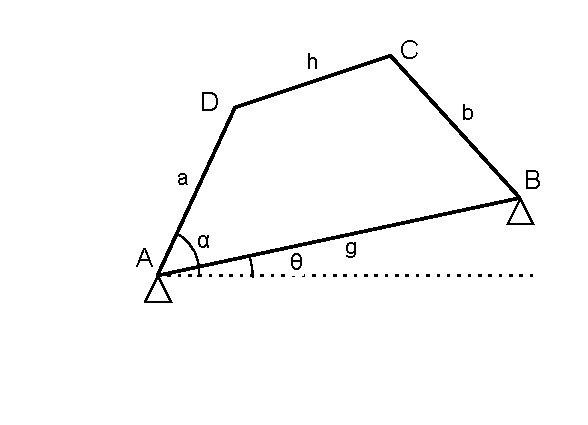
\includegraphics[width=\linewidth]{./figures/four-bar_linkage.pdf}
	    \caption{Planar four-bar linkage}
	    \label{fig:linkage-1}
	\end{subfigure}
	\hfill
	\begin{subfigure}{0.49\textwidth}
		\centering
		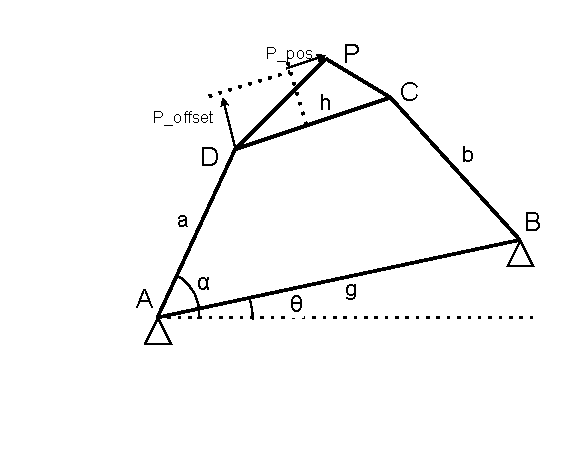
\includegraphics[width=\linewidth]{./figures/four-bar_linkage+coupler.pdf}
		\caption{Planar four-bar linkage with coupler $P$}
		\label{fig:linkage-2}
	\end{subfigure}
	\caption{Four-bar linkage}
\end{figure}

To provide a comprehensive overview, this report is structured as follows. In Section \ref{ch:analysis}, we discuss and analyze user requirements, derive system requirements, and provide a theory foundation for the geometry of the linkage. Section \ref{ch:design} covers the selection of implementation environment based on the task and team's expertise, followed by the design of UML class diagrams to be used during implementation. After that, in Section \ref{ch:implementation}, we implement the four-bar linkage model, the graphical user interface (GUI), and the test cases. In Section \ref{ch:validation}, we assess the correctness of the implementation by testing all possible motion types of the linkage. Section \ref{ch:optimization-problem} provides a solution to the problem of moving a box along a conveyor under certain constraints. Finally, in Sections \ref{ch:doc} and \ref{ch:projectmanagement}, we describe the software documentation and the project management.

\section{Analysis} \label{ch:analysis}

\subsection{User Requirements}\label{ch:user_requirements}

\begin{figure}[h]
	\centering
	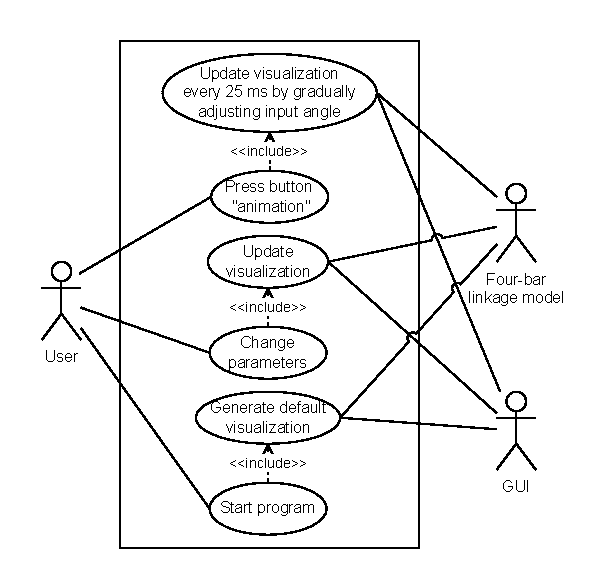
\includegraphics[width=0.7\textwidth]{./figures/uml_use_case.pdf}
	\caption{UML use case diagram}
	\label{fig:use_case}
\end{figure}

User requirements are a list of customer expectations that the software must fulfill after development. These requirements are normally high-level expectations, that need to be translated by the developers into technical system requirements.

To better understand the user requirements listed below, we provide a UML use case diagram in Figure \ref{fig:use_case}. The diagram illustrates the user-software interaction. After the user starts the GUI, the software generates the default visualization of the four-bar linkage. The user also has an option to enter new geometric parameters and obtain the updated visualization. Moreover, if the user enables animation mode, the four-bar linkage model gradually increases the input angle and the GUI updates the visualization every $25$ milliseconds with new geometric data to simulate the motion of the linkage.

The following list contains all the user requirements provided by our supervisor, supplemented with our explanation for each.

\begin{itemize}
	\item \textit{Requirement: Implement all motion types of a planar four-bar linkage extended with a coupler.}
	
	Figure \ref{fig:linkage-2} illustrates the four-bar linkage with a coupler, which will be implemented in this work. As explained in \cite{inproceedings}, there are $27$ distinct motion cases of the planar four-bar linkage. All of the motion cases and corresponding geometry will be explained in the next sections.
	
	\item \textit{Requirement: Implement a graphical user interface (GUI) to display and animate the four-bar linkage, and to input geometric parameters.}
	
	The GUI should provide the visualization of the four-bar linkage with a coupler, as well as the animation of its motion. User should have an option to configure the linkage parameters using the GUI. We have identified ten free geometric parameters (degrees of freedom), that the GUI should support:
	
	\begin{itemize}
		\item The lengths of the four bars ($AB$, $BC$, $CD$, $AD$).
		\item The angle $\theta$ between the fixed bar $AB$ and the horizontal line.
		\item The input angle $\alpha$ between the bar $AD$ and the horizontal line.
		\item The position of the coupler relative to the middle of the floating link $CD$, expressed by $P_{pos}$ and $P_{offset}$.
		\item Position of the joint $A$ on xy-plane (x- and y-coordinates).
	\end{itemize}
	
	For animation, the input angle $\alpha$ is no longer a free parameter, because it will be dynamically adjusted by the system to simulate the motion of the linkage.
	
	Also note that, for simplicity, we will fix the joint $A$ at $(0, 0)$ for analysis and visualization in the GUI. To change the position of $A$, we will translate the entire linkage accordingly. The configurable position of $A$ will be important to solve an optimization problem discussed in the next point.
	
	\item \textit{Requirement: Find the four-bar linkage with a coupler to solve the following optimization problem:}
	\begin{itemize}
		\item Push the box with size $80\times60$ from $x=220$ to $x=0$
		\item Do not cross the area of the labeling machine (area where $x<80$ and $y>70$).
		\item Pass above the points $(120, 80)$ and $(220, 80)$
	\end{itemize}
	
	\begin{figure}[h]
		\centering
		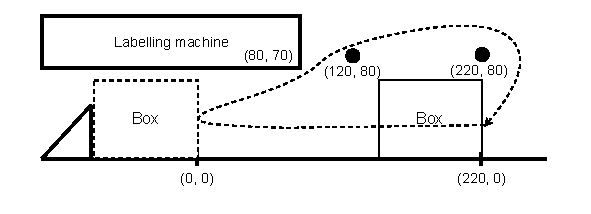
\includegraphics[width=0.7\textwidth]{./figures/optimization_problem_task.pdf}
		\caption{Optimization problem}
		\label{fig:optimization_problem}
	\end{figure}
	
	Figure \ref{fig:optimization_problem} illustrates the optimization problem. To solve the problem we need to find the geometrical parameters of the linkage, so that the coupler P will move the box along the conveyor line, avoiding all obstacles, and then return for the next box. The example trajectory of $P$ is depicted as the dotted line.
	
	The minimum requirement is to solve this problem manually by experimenting to find a suitable linkage. Ideally, we would develop an algorithm to find suitable parameters efficiently.
\end{itemize}

\subsection{System Requirements}

After discussing the user requirements, which provide only a high-level overview of the software, we need to derive more technical system requirements. The system requirements are subdivided into functional requirements, which describe what system should do, and non-functional requirements, which specify how the system should meet the functional requirements.

We begin with the functional requirements.

\begin{itemize}
	\item \textit{Four-bar linkage model:}
	\begin{itemize}
		\item The model calculates joints' coordinates based on the input parameters.
		\item It implements all 27 motion types of the four-bar linkage with a coupler.
		\item It validates the user's input.
		\item It ensures stable operation without crashes.
	\end{itemize}
	
	The four-bar linkage model is a back-end part of the software, which implements the geometry and all motion types of the four-bar linkage. Its role is to provide correct data for visualization and animation of the linkage in the GUI. The model validates the input data and notifies the GUI, prompting the user to change an invalid input.
	
	\item \textit{Tests:}
	\begin{itemize}
		\item Implement test cases for all motion types of the four-bar linkage.
		\item Provide reference data.
	\end{itemize}
	
	To guarantee the back-end's accuracy, we must implement test cases for each motion type and provide appropriate reference data.
	
	\item \textit{Graphical User Interface (GUI):}
	\begin{itemize}
		\item The GUI uses the four-bar linkage model (back-end) to get the coordinates of the joints for visualization and animation.
		\item It provides a visualization of the four-bar linkage.
		\item It contains sliders for user to input geometric parameters.
		\item It updates the visualization according to the user's input.
		\item It includes an animation mode for smooth motion visualization of the four-bar linkage.
		\item It provides tracing of the trajectory for the coupler.
	\end{itemize}
	
	The GUI is the front-end interface for the user to generate the visualization and animation of the linkage based on the user's input. It uses data obtained from the four-bar linkage model. Therefore, the user must be able to input parameters in the GUI. To solve the optimization problem, we also need to trace the motion of the coupler.
	
	\item \textit{Documentation}
	\begin{itemize}
		\item The four-bar linkage model, tests, and GUI are documented in detail.
	\end{itemize}
	
	High-quality documentation is essential for code to be reusable and maintainable.
\end{itemize}

Since we have defined the functional system requirements, we define now the non-functional system requirements.

\begin{itemize}
	\item \textit{Performance:}
	\begin{itemize}
		\item The four-bar linkage model must provide smooth animations.
		\item The GUI animations should run at a minimum of 30 frames per second. 
	\end{itemize}
	
	The crucial factor for usability of the software is its performance. In our case, performance is measured by the number of frames per second (fps) during the animation. This criterion also depends on the machine used to run the code, so we assess the fps using a standard laptop with an AMD Ryzen 5 4500U chip.   
\end{itemize}

\subsection{Geometry}\label{ch:geometry}

After analyzing the user requirements and deriving system requirements, we focus on the geometry of the given linkage. This will be implemented as part of the four-bar linkage model and used to create visualization and animation later in the GUI.

To visualize the linkage, we need to calculate the positions of all the joints based on the input parameters. The input parameters are:
\begin{itemize}
 \item The lengths of main four bars $AB$, $BC$, $CD$, $AD$, that we denoted as $g$, $b$, $h$, $a$.
 \item The input angle $\alpha$.
 \item The angle $\theta$ between the horizontal line and $AB$.
 \item The position of coupler $P$ defined with respect to midpoint of $CD$ and denoted as $P_{pos}$ and $P_{offset}$. 
 
 Note that these two values also can be negative, take a look at the direction of corresponding arrows in Figure \ref{fig:four-bar_linakge_analysis}.
\end{itemize}

All the mentioned parameters are depicted in Figure \ref{fig:four-bar_linakge_analysis}.

\begin{figure}[h]
	\begin{center}
		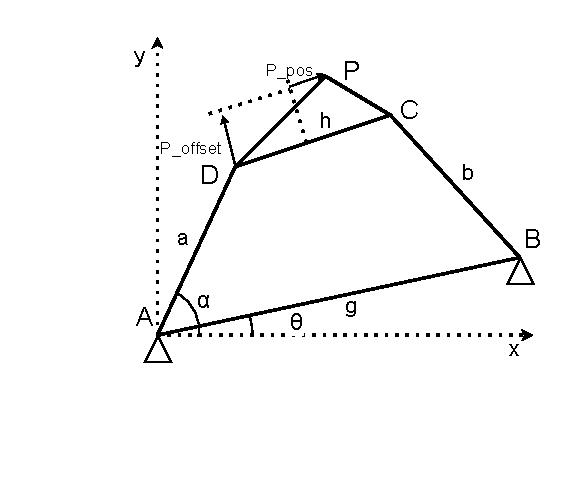
\includegraphics[width=0.5\textwidth]{./figures/four-bar_linkage+coupler_analysis.pdf}
	\end{center}
	\caption{Planar four-bar linkage with coupler $P$}
	\label{fig:four-bar_linakge_analysis}
\end{figure}
 
 After recalling all the input parameters we use them to find out the positions of the joints one by one.
 
 \begin{itemize}
 	\item Joint $A$.
 	
 	As previously mentioned, we position joint $A$ at $(0, 0)$ for simplicity. To place it at different coordinates, the whole linkage should be translated by adding the new coordinates of $A$ to each joint's coordinates.
 	
 	\item Joint $B$.
 	
 	The position of joint $B$ can be defined using $g$, the length of bar $AB$, and angle $\theta$: $B_x = g  \cos(\theta)$, $B_y = g \sin(\theta)$.
 	
 	\item Joint $D$.
 	
 	The position of joint $D$ is also easy to determine using $a$, the length of $AD$, and input angle $\alpha$: $D_x = a \cos(\alpha)$, $D_y = a \sin(\alpha)$.
 	
 	\item Joint $C$.
 	
 	The most complex problem is to determine the position of joint $C$. The main idea is to derive the position of $C$ by considering the area of triangle $\triangle BCD$ using different methods.
 	
 	To determine the position of $C$, we consider new basis vectors.
 	
 	Define a vector $\overrightarrow{BD} = (BD_x, BD_y) = \overrightarrow{D} - \overrightarrow{B} = (D_x - B_x, D_y - B_y)$. Assume first that this vector has non-zero length $|\overrightarrow{BD}| = \sqrt{(BD_x)^2+(BD_y)^2}$. 
 	
 	The corresponding unit vector along $\overrightarrow{BD}$ is $\overrightarrow{e}_{BD} = (e_{BD_-x}, e_{BD_-y}) = \frac{\overrightarrow{BD}}{|\overrightarrow{BD}|}$.
 	
 	The orthogonal direction is defined by a unit vector $\overrightarrow{n}_{BD} = (-e_{BD_-y}, e_{BD_-x})$.
 	
 	We use the vectors $\overrightarrow{e}_{BD}$ and $\overrightarrow{n}_{BD}$ as a new orthonormal basis.
 	
 	To determine the area of $\triangle BCD$ we use Heron's formula:
 	
 	$A_{\triangle BCD} = \sqrt{p (p-b) (p-h) (p-|\overrightarrow{BD}|)}$, where $p = \frac{b + h + |\overrightarrow{BD}|}{2}$ is a semi-perimeter of $\triangle BCD$.
 	
 	On the other hand the area of $\triangle BCD$ can be determined using length of $BD$ and the perpendicular from $C$ to $BD$ denoted by $C_{offset}$ (see Figure \ref{fig:four-bar_linakge_analysis}): $A_{\triangle BCD} = \frac{|\overrightarrow{BD}| C_{offset}}{2}$. So we can determine $C_{offset} = 2 \frac{A_{\triangle BCD}}{ |\overrightarrow{BD}|}$
 	
 	At this point, we know the distance from joint $C$ to $BD$ along $\overrightarrow{n}_{BD}$. To determine the position of $C$ with respect to $B$, we also need the distance from $C$ to $B$ along $\overrightarrow{e}_{BD}$. The projection length of $\overrightarrow{BC}$ onto direction of $\overrightarrow{e}_{BD}$ is given by $|C_{pos}| = \sqrt{b^2 - C_{offset}^2}$ using Pythagorean theorem. The remaining question is to determine sign of this projection. This can be done using angle $\angle CBD$ and the Law of Cosines: 
 	
 	$\cos(\angle CBD) = \frac{b^2 + |\overrightarrow{BD}|^2 - h^2}{2 b |\overrightarrow{BD}|}$
 	
 	Then the projection of $\overrightarrow{BC}$ onto direction of $\overrightarrow{e}_{BD}$ is given by $C_{pos} = sign(\cos(\angle CBD)) \sqrt{b^2 - C_{offset}^2}$
 	
 	After determining $C_{pos}$ and $C_{offset}$, we can find the possible positions of $C$:
 	
 	$\overrightarrow{C}_1 = (C_{1_-x}, C_{1_-y}) = \overrightarrow{B} + C_{pos} \overrightarrow{e}_{BD} + C_{offset} \overrightarrow{n}_{BD}$ 
 	
 	$\overrightarrow{C}_2 = (C_{2_-x}, C_{2_-y}) = \overrightarrow{B} + C_{pos} \overrightarrow{e}_{BD} - C_{offset} \overrightarrow{n}_{BD}$
 	
 	There are two possible positions of $C$, because the normal vector to $\overrightarrow{BD}$ is not unique and can also have the opposite direction. For a static structure, we can choose any of them, so we take $C = C_2$ as the default. For the animation case, that will be discussed later, there are rules for choosing between $C_1$ and $C_2$.
 	
 	In the discussion above we made the assumption that the length of $\overrightarrow{BD}$ is not zero. However, for $b = h$ and a specific value of input angle $\alpha$, the length can become zero. In this case, the joints $A$, $B$, $C$, $D$ are on the same line, so we define a unit vector $\overrightarrow{e} = sign(\overrightarrow{BA} \cdot \overrightarrow{BC})\frac{\overrightarrow{BA}}{g}$, where $\cdot$ is a scalar product. Then, the position of $C$ is determined uniquely by $\overrightarrow{C} = \overrightarrow{B} + b \overrightarrow{e}$
 	
 	\item Coupler $P$.
 	
 	Since we know the positions of $C$ and $D$, it is easy to determine the position of $P$.
 	
 	Define the midpoint of $CD$ as $\overrightarrow{Q} = \frac{\overrightarrow{C} + \overrightarrow{D}}{2}$.
 	
 	The unit vector along $DC$ is given by $\overrightarrow{e}_{DC} = (e_{DC_-x}, e_{DC_-y}) = \frac{\overrightarrow{C} - \overrightarrow{D}}{h}$. The corresponding normal vector is $\overrightarrow{n}_{DC} = (-e_{DC_-y}, e_{DC_-x})$.
 	
 	Then, the position of the coupler $P$ is determined by $\overrightarrow{P} = \overrightarrow{Q} + P_{pos} \overrightarrow{e}_{DC} + P_{offset} \overrightarrow{n}_{DC}$.
 	
 	Unlike the position of $C$, the position of $P$ is determined uniquely, because $P_{offset}$ can be specified as negative by the user, automatically changing the direction of $\overrightarrow{n}_{DC}$.
 \end{itemize}

 \subsection{Parameter Validation}
 
 Not every set of the input parameters is feasible. In this section we will derive constraints on the input angle $\alpha$ and the links' lengths to ensure that the linkage exists.
 
 \begin{figure}[h]
 	\centering
 	\begin{subfigure}{0.3\textwidth}
 		\centering
 		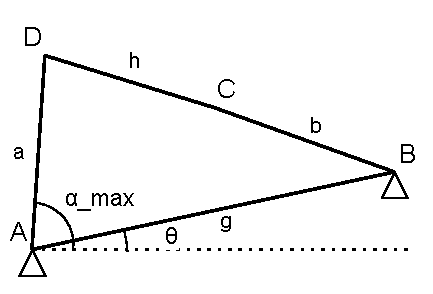
\includegraphics[width=\linewidth]{./figures/linkage_input_angle_limits_1.pdf}
 		\caption{Maximum input angle $\alpha$.}
 		\label{fig:max_alpha}
 	\end{subfigure}
 	\hfill
 	\begin{subfigure}{0.3\textwidth}
 		\centering
 		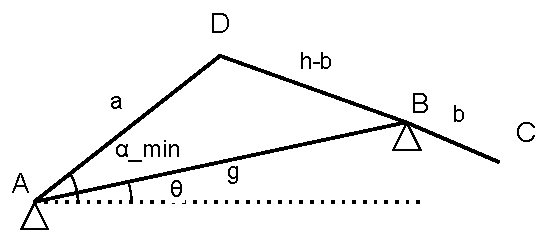
\includegraphics[width=\linewidth]{./figures/linkage_input_angle_limits_2.pdf}
 		\caption{Minimum input angle $\alpha$.}
 		\label{fig::min_alpha-1}
 	\end{subfigure}
 	\hfill
 	\begin{subfigure}{0.3\textwidth}
 	\centering
 	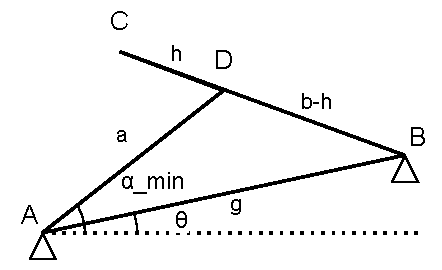
\includegraphics[width=\linewidth]{./figures/linkage_input_angle_limits_3.pdf}
 	\caption{Minimum input angle $\alpha$.}
 	\label{fig::min_alpha-2}
 	\end{subfigure}
 	\caption{Constraints on the input angle $\alpha$.}
 \end{figure}
 
 Figures \ref{fig:max_alpha}, \ref{fig::min_alpha-1}, \ref{fig::min_alpha-2} illustrate the cases of the maximum and minimum input angle $\alpha$. The coupler $P$ has no influence on the limits of the input angle therefore it is not shown in the figures. The limits of $\alpha$ are defined by the cases when the four-bar linkage folds into a triangle.
 
 \begin{itemize}
 \item Maximum input angle $\alpha$.
 
 Figure \ref{fig:max_alpha} displays the upper limit of the angle $\alpha$, that can be derived using the Law of Cosine for triangle $\triangle ABD$: $(h+b)^2 = a^2 + g^2 - 2 a g \cos(\alpha_{max}-\theta)$.
 
 If this cosine $\cos(\alpha_{max}-\theta) = \frac{a^2 + g^2 - (h+b)^2}{2 a g}$ has an absolute value less than one, there exists an upper limit for the input angle $\alpha$: $\alpha_{max} = \arccos(\frac{a^2 + g^2 - (h+b)^2}{2 a g}) + \theta$.
 
 \item Minimum input angle $\alpha$.
 
 Figures \ref{fig::min_alpha-1}, \ref{fig::min_alpha-2} show two different cases for minimum input angle $\alpha$. The both cases could be described using the Law of Cosine for triangle $\triangle ADB$: $(h-b)^2 = a^2 + g^2 - 2 a g \cos(\alpha_{min}-\theta)$.
 
 If this cosine $\cos(\alpha_{min}-\theta) = \frac{a^2 + g^2 - (h-b)^2}{2 a g}$ has an absolute value less than one, there exists a lower limit of the input angle $\alpha$: $\alpha_{min} = \arccos(\frac{a^2 + g^2 - (h-b)^2}{2 a g}) + \theta$.
 
 \item Special cases.
 
 If both cosines $\cos(\alpha_{min}-\theta)$ and $\cos(\alpha_{max}-\theta)$ have an absolute value greater or equal one, then there is no limits to the input angle $\alpha$.
 
 If only the maximum limit exists, then the input angle $\alpha$ also has a lower boundary, that is symmetric with respect to the ground link $AB$: $\alpha \in [\alpha_{max}, 2 \theta - \alpha_{max}]$.
 
 In the opposite case, when only the minimum input angle $\alpha$ exists, then the input angle is also bounded from above symmetrically with respect to the ground link $AB$: $\alpha \in [2 \theta + 2 \pi - \alpha_{min}, \alpha_{min}]$.
 \end{itemize}
 
 We decided that the GUI will display a slider for input angle $\alpha$, ensuring that only valid values within the boundaries can be entered by the user. A similar limitation can be derived for the output angle $\angle ABC$.
 
 There is also a case when the four-bar linkage does not exist for any input angle $\alpha$. This occurs when one of the bars is longer than the sum of other three, so that the quadrilateral $\square ABCD$ does not exist. Denote the longest bar as $l = \max(a, b, g, h)$, the shortest bar as $s = \min(a, b, g, h)$, and two remaining bars as $p$, $l$. Then the condition for linkage to exist is $l-p-q-s \le 0$. This condition will be checked by the four-bar linkage model, which will notify the user through the GUI in case of a problem.
 

 \subsection{Classification}
 
 After deriving the expressions for constraints on the input angle $\alpha$, we can classify the motion of four-bar linkage.
 
 Depending on the constraints on the input angle $\alpha$ and the output angle $\angle ABC$, the input link $AD$ and the output link $BC$ can be classified into four types according to \cite{inproceedings}.
 
 \begin{itemize}
 	\item \textit{Crank}.
 	
 	The link can rotate fully, with neither a minimum, nor a maximum for the input angle $\alpha$ (or the output angle $\angle ABC$).
 	
 	\item \textit{Rocker}.
 	
 	The link can rotate partially, with both a minimum and a maximum for the input angle $\alpha$ (or the output angle $\angle ABC$).
 	
 	\item \textit{0-rocker}.
 	
 	The link can rotate partially, with no minimum but with maximum for the input angle $\alpha$ (or the output angle $\angle ABC$).
 	
 	\item \textit{$\pi$-rocker}.
 	
 	The link can rotate partially, with no maximum but with minimum for the input angle $\alpha$ (or the output angle $\angle ABC$).
 \end{itemize}
 
 \subsection{27 Motion Types}\label{ch:27_motion_types}
 
 The classification of the input and output links implies, that there are different linkage types. For example, the input and output can independently be classified as cranks or rockers, leading to different linkage types. The study in \cite{inproceedings} identifies $27$ different combinations. These combinations can be described by signs of characteristic values: $T_1 = g + h - a - b$, $T_2 = b + g - h - a$ and $T_3 = b + h - g - a$. Since each characteristic value can be positive, negative, or zero, there are $27$ possible combinations and motion types respectively.
 
 Initially, we discussed to analyze the motion in each of $27$ cases separately. However, we decided to implement the general algorithms that handles all cases.
 

 \subsection{Animation}\label{ch:animation}

 At the beginning of the animation, we start with a static state of the linkage. By default we set $C_2$ as the chosen position for joint $C$.
 The animation is implemented as a discrete process by gradually incrementing the input angle using the following key variables:
 \begin{itemize}
 	\item $dt$: Time interval of the animation.
 	\item $\dot{\alpha}$: constant angular velocity of the input angle $\alpha$.
 \end{itemize}

This is our basic idea of iterative animation:
\begin{itemize}
	\item Calculate the limit values of $\alpha$ described above.
	
	\item Update $\alpha$ using the following formula: $\alpha = \alpha \pm \dot{\alpha} dt$.
		 
	The sign here depends on the \texttt{direction} parameter. It determines whether $\alpha$ changes clockwise (\texttt{direction = 1}) or counterclockwise (\texttt{direction = 0}).
	 
	\item Use the updated $\alpha$ value to calculate other parameters, such as the positions of the joints.
		 
	\item If the input angle $\alpha$ is limited, then change the \texttt{direction} parameter at the limits to rotate the input link backwards.
		 
	\item If the input angle is not bounded, ensure that $\alpha$ always remains within the range $[0^\circ, 360^\circ]$. If the input angle exceeds $360^\circ$ or falls below $0^\circ$, we will reset it to the corresponding boundary value.
		 
	\item Switch between $C_1$ and $C_2$ to ensure continuity of animation.
	
	As we mentioned earlier, for the static configuration, we choose $C_2$ as the default position for joint $C$. However, during the motion, we need to switch between $C_1$ and $C_2$ to maintain continuous velocity due to the principle of inertia. This means that at every limit of the input angle we switch between $C_1$ and $C_2$.
	
	Note, that we need to switch even at the boundary cases, when the absolute values of $\cos(\alpha_{max}-\theta)$ or $\cos(\alpha_{min}-\theta)$ are equal to one, indicating that the input angle has reached its extreme positions.

	\item Consider floating point precision.
	
	To avoid issues caused by floating point inaccuracies when checking if the cosine value of $\alpha$ approaches $-1$ or $1$, we incorporate floating point tolerance of $10^{-10}$.
\end{itemize}

We also created a UML statechart diagram for the animation algorithm that can be found in Figure \ref{fig:state_diagramm_of_animation_alpha} in the Appendix.

%\begin{figure}[h]
%    \centering
%    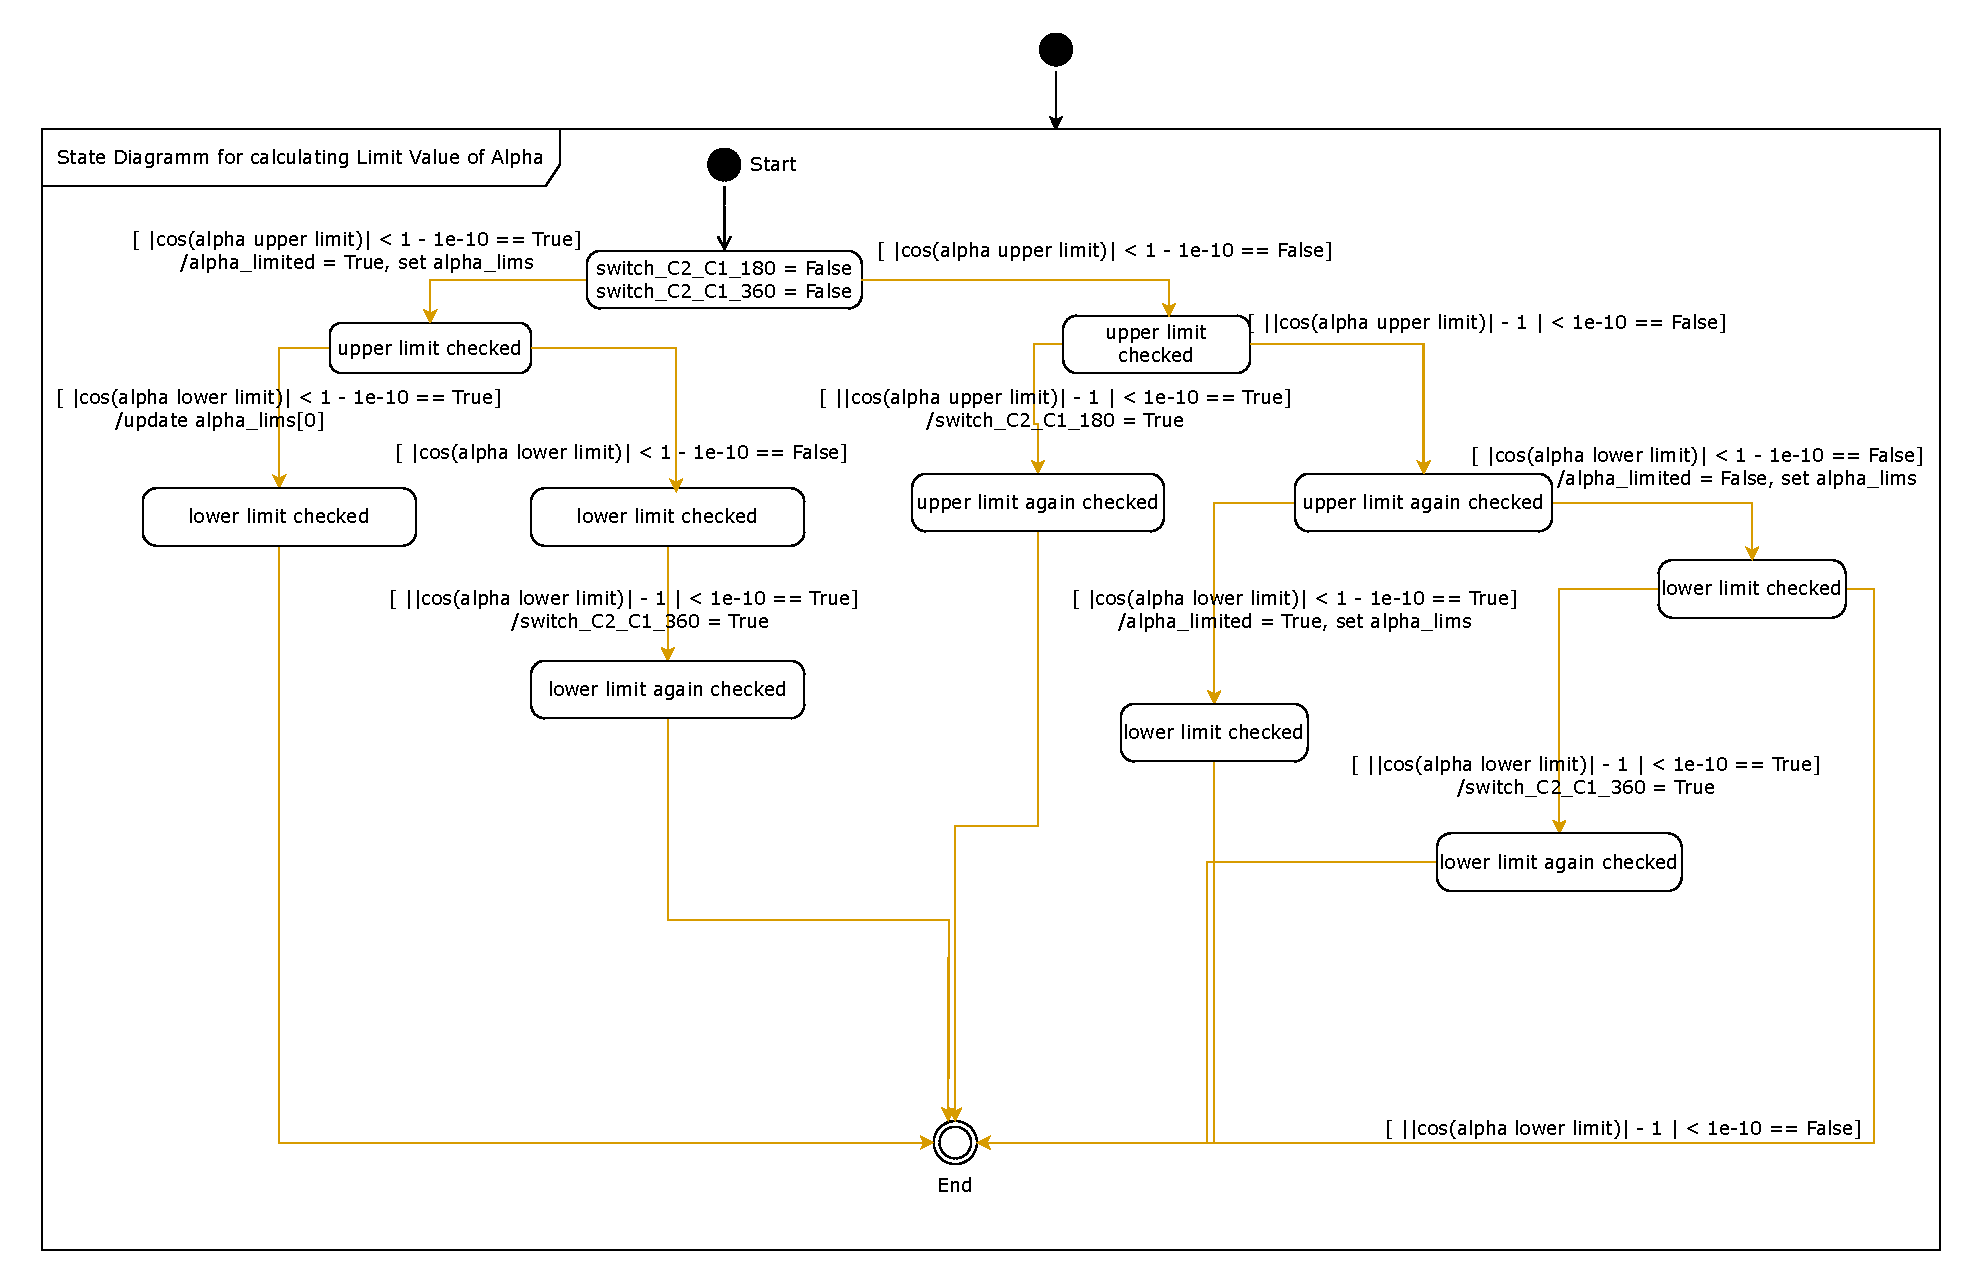
\includegraphics[width=\textwidth]{./figures/state_diagramm_calculate_alpha_limit_1.pdf}
%    \caption{State Diagramm for calculating Alpha Limit}
%    \label{fig:state_diagramm_calculate_alpha_limit}
%\end{figure}

%\textbf{Figure \ref{fig:state_diagramm_calculate_alpha_limit} %shows the algorithm we designed:}
%\begin{itemize}
%    \item Firstly, it determines whether \(\alpha\) is limited (e.g., \(|\cos(\text{alpha upper limit})| < 1 - 10^{-10}\)).
%    \item Secondly, it checks whether the extreme values of \(\alpha\) are exactly \(0^\circ\), \(180^\circ\), or \(360^\circ\) (e.g., \(\bigl|\bigl| \cos(\text{alpha lower limit}) \bigr| - 1 \bigr| < 10^{-10}\)). Here, \(10^{-10}\) is the floating point tolerance that we used.
%    \item Based on this, it sets the parameters \(\text{switch\_C2\_C1\_180}\) and \(\text{switch\_C2\_C1\_360}\), which indicates whether there is a need to switch \(\alpha\) at these special values.
%\end{itemize}



\section{Design} \label{ch:design}

After completing the analysis part we begin to design the software that will be implemented later. Our design section consists of two parts, the selection of development infrastructure and the creation of class diagrams to be a basis for implementation.

\subsection{Third-Party Software and Development Infrastructure}

Since we now understand the problem that we need to solve, we can choose an implementation environment.

We decided to implement our project using Python. This decision is based on several key factors:
\begin{itemize}
	\item Python has a numpy\footnote{\label{fn:numpy} \url{https://numpy.org/}} library that deals well with vector operations. The four-bar linkage model requires solving geometrical problem, so the built-in vector and matrix operations are highly desired to simplify the code.
	\item Python has a standard GUI library tkinter\footnote{\label{fn:tkinter} \url{https://docs.python.org/3/library/tkinter.html}}.
	\item Most of the team members have more experience with Python than with C++.
\end{itemize}

There is a list of the software and tools we used for implementation:
\begin{itemize}
	\item Operating systems: Xubuntu and Windows.
	\item Programming language: Python.
	\item Integrated development environment (IDE): Spyder\footnote{\url{https://www.spyder-ide.org/}} and PyCharm\footnote{\url{https://www.jetbrains.com/pycharm/}}.
	\item Package manager: Anaconda\footnote{\url{https://www.anaconda.com/}}.
	\item Libraries: tkinter\textsuperscript{\ref{fn:tkinter}}, numpy\textsuperscript{\ref{fn:numpy}}, math\footnote{\url{https://docs.python.org/3/library/math.html}}, unittest\footnote{\url{https://docs.python.org/3/library/unittest.html}}.
	\item Version control system: GitHub repository\footnote{\url{https://github.com/einsflash/Project_Pusher_Mechanism}}.
	\item Documentation: Pdoc\footnote{\url{https://pdoc.dev/docs/pdoc.html}}.
\end{itemize}

\subsection{Class Models}

In the project we need to store a large amount of variables for geometric representation and visualization of the four-bar linkage, as well as for corresponding tools like buttons und sliders. The number of variables is too large to pass it into different functions as arguments. Therefore, we decided to implement the four-bar linkage model and the GUI as two separate classes, so every member function will have an access to the data stored in the class without passing it as an argument.

\begin{figure}[h]
	\begin{center}
		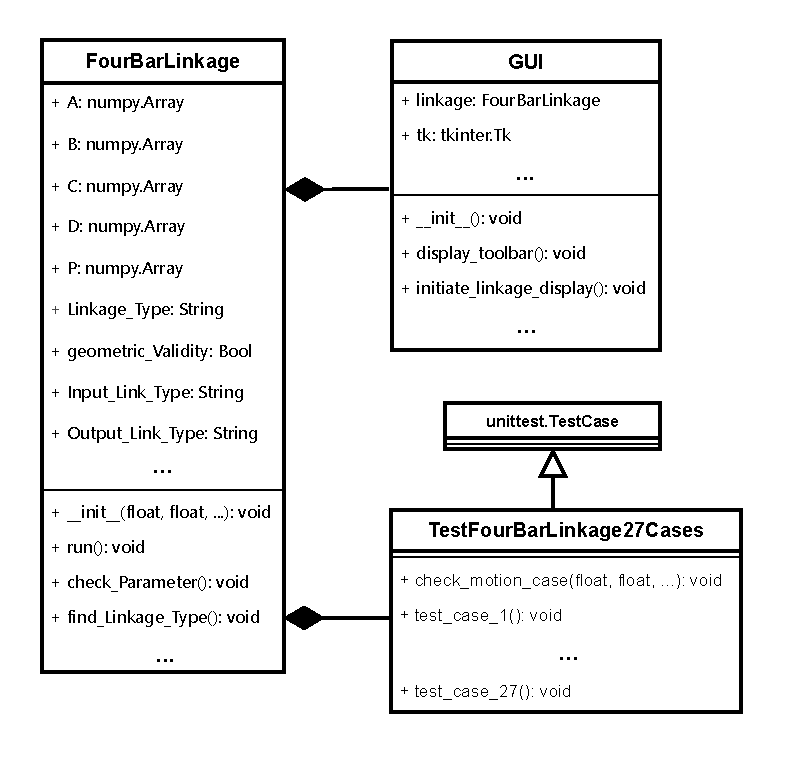
\includegraphics[width=0.65\textwidth]{./figures/class_diagram.pdf}
	\end{center}
	\caption{UML class diagram}
	\label{fig:class diagram}
\end{figure}

Figure \ref{fig:class diagram} shows a shortened version of the class diagram. This diagram illustrates all the relationships between classes and the most important attributes. The actual number of attributes is too high to include it in this document, the comprehensive class diagram can be found in our GitHub repository\footnote{\url{https://github.com/einsflash/Project_Pusher_Mechanism/blob/main/src/class_diagram.pdf}}.

The back-end class \texttt{FourBarLinkage} implements the geometry and animation of the four-bar linkage with a coupler. The number of member variables is large, but the most important for visualization are the coordinates of joints $A$, $B$, $C$, $D$, and $P$. There are also member variables used for classification (\texttt{Linkage\_Type}, \texttt{Input\_Link\_Type}, \texttt{Output\_Link\_Type}) and for input validation (\texttt{geometric\_Validity}) to notify GUI about invalid parameters. The main member functions are the constructor \texttt{\_\_init\_\_} to set geometrical parameters, \texttt{run} to compute the joints' coordinates, \texttt{check\_Parameter} to validate user input, and \texttt{find\_Linkage\_Type} to classify the linkage. There are many other attributes used for internal purposes, but they are less important for a general overview.

The front-end class \texttt{GUI} is used to create the graphical user interface to visualize linkage, provide its animation and get geometrical parameters from the user. This class has also a large number of attributes, but only several of them are important for an overview. The member variables include an instance of the \texttt{FourBarLinkage} class, which is used to obtain joint coordinates for visualization and animation. The \texttt{GUI} class also contains an instance of \texttt{tkinter.Tk}, the basic class for creating GUI using tkinter. The main member functions are the constructor \texttt{\_\_init\_\_} to initiate the GUI, \texttt{display\_toolbar} to set up the toolbar of buttons, sliders, and other elements, and \texttt{initiate\_linkage\_display} to set up the visualization of the linkage.

The test class \texttt{TestFourBarLinkage27Cases} inherits from \texttt{unittest.TestCase} and is used to test all motion types of the linkage. This class has only member functions that implement test cases for each motion types.

\section{Implementation} \label{ch:implementation}

\subsection{Back-End}
The back-end class \texttt{FourBarLinkage} contains the implementation of the four-bar linkage, specifically its geometric description, which is used by the GUI for visualization and animation. The back-end is implemented using the numpy and math packages for efficient calculations. The implementation strictly follows the design and analysis phases. Details about the four-bar linkage were thoroughly explained in Section \ref{ch:analysis}, so we will not repeat them here.

First, we implemented the linkage classification table from the paper \cite{inproceedings} as a dictionary in the function \texttt{find\_Linkage\_Type}, and then used the classification values $T_1$, $T_2$, and $T_3$ to determine the linkage type. Afterwards we implemented a function that allows to input the classification values instead of link lengths, that is especially useful during the testing phase. Moreover, we implemented all the geometry of the four-bar linkage and animation algorithm.

As an interface for the GUI, we created a function \texttt{run}, which integrates all geometry and animation functions. This function is triggered by the GUI to recalculate the joint positions when the input parameters are updated or during animation.

The overview of the \texttt{FourBarLinkage} class can be found in the documentation\footnote{\url{https://htmlpreview.github.io/?https://github.com/einsflash/Project_Pusher_Mechanism/blob/main/src/doc_for_four_bar_linkage/four_bar_linkage.html}}.

\subsection{Front-End}

After considering the back-end part of the software that implements the geometry of the four-bar linkage extended with a coupler, we focus on the GUI. The GUI will use the back-end to visualize the linkage and simulate its animation, enabling the user to adjust geometrical parameters of the linkage. The GUI is implemented using tkinter\textsuperscript{\ref{fn:tkinter}}. We will not go into too many details about the implementation to keep the description concise.

\begin{figure}[h]
	\begin{center}
		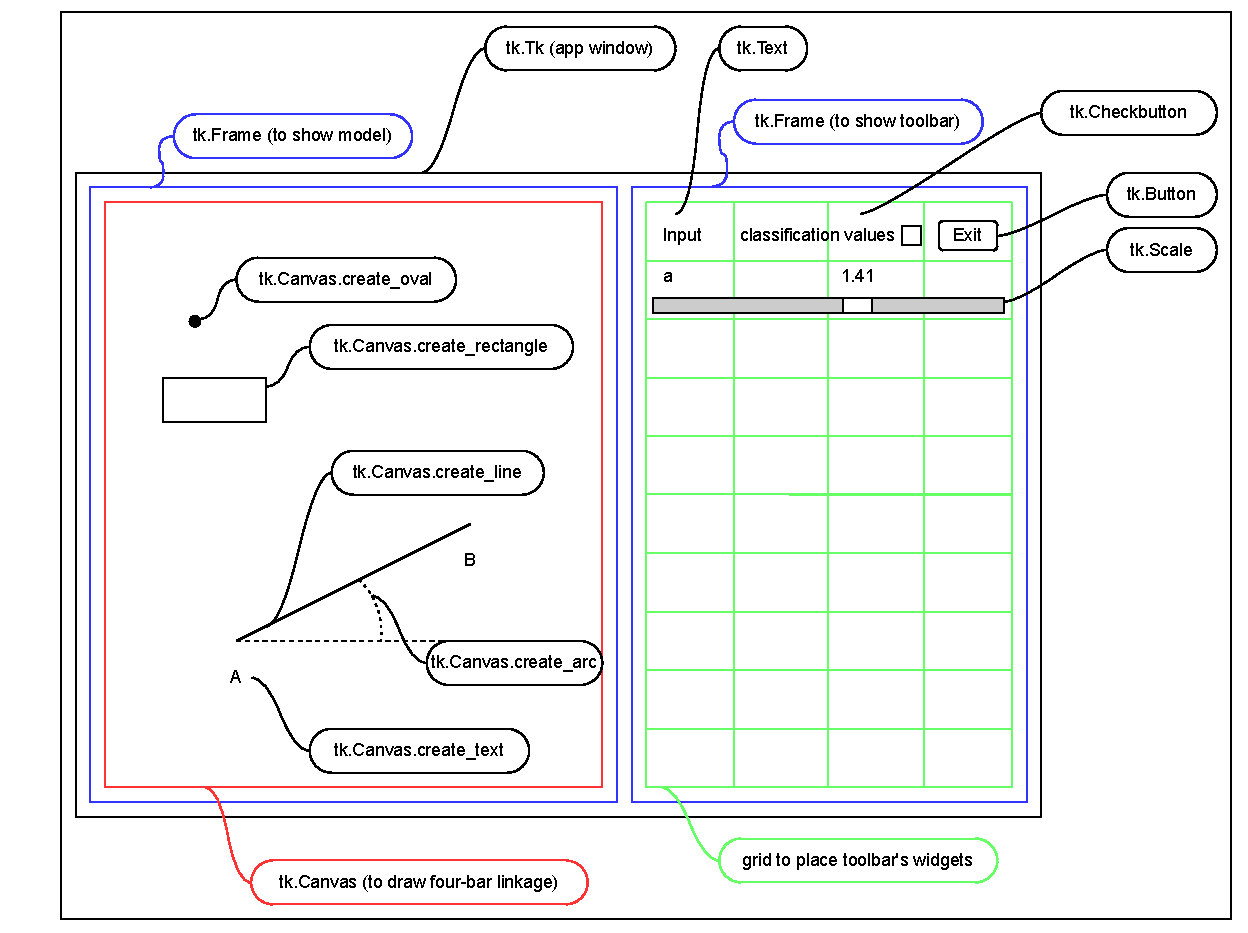
\includegraphics[width=0.7\textwidth]{./figures/tkinter_grid.pdf}
	\end{center}
	\caption{The main components of the GUI.}
	\label{fig:tkinter_parts}
\end{figure}

The main components of the GUI are illustrated in Figure \ref{fig:tkinter_parts}. The components of the tkinter are widgets that can be displayed in the GUI. The basic object of the GUI is \texttt{tkinter.Tk}. All other widgets are placed in the GUI using \texttt{tkinter.Frame} widget, which creates a grid and allows the explicit specification of widget positions.

The GUI is divided into two parts by two \texttt{tkinter.Frame} objects. The left one is used to generate the visualization of the linkage. It holds a singe widget, \texttt{tkinter.Canvas}, which can display all the basic geometric figures and text. The positions of these figures are specified using pixel-based x-y coordinates. The right \texttt{tkinter.Frame} is used to display the toolbar. The widget's position in the toolbar is specified using the grid. The toolbar is used to enter new geometrical parameters using the sliders \texttt{tkinter.Scale}. The toolbar also allows the user to change the visualization mode, e.g. enabling animation or tracing, using \texttt{tkinter.Button} and \texttt{tkinter.Checkbutton} objects.

To start the GUI, we call \texttt{tkinter.Tk.mainloop}.

The GUI needs the coordinates of the joints to visualize the linkage on \texttt{tkinter.Canvas}. To achieve that, the GUI contains the \texttt{FourBarLinkage} object as a member variable. To calculate the joints' coordinates, the GUI calls the back-end's member function \texttt{FourBarLinkage.run} and extracts the positions using the back-end's member variables \texttt{FourBarLinkage.A}, \texttt{FourBarLinkage.B}, and so on. These coordinates are scaled to fit the GUI's screen resolution, and then each link of the four-bar linkage is visualized using the \texttt{tkinter.Canvas.create\_line} function.

For animation, we use \texttt{tkinter.Tk.after(25, func)}, which calls the \texttt{func} function after $25$ milliseconds, allowing to update the visualization of the linkage in a loop.

To respond to the new geometric parameters entered by the user using the slider \texttt{tkinter.Scale}, each slider is linked to a specific function, called after each change of the value. For example, the slider used to set $a$ is linked to the function \texttt{update\_parameter\_a}: 

\begin{lstlisting}
def update_parameter_a(self, val):
	self.linkage.DA = float(val)
	self.delete_tracing()
	self.refresh()
\end{lstlisting}

This function reads the new value of $a$ stored in the \texttt{val} variable, and updates the geometric parameter $AD$ in the linkage accordingly. It also calls the \texttt{delete\_tracing} function to remove no longer relevant trajectory visualization for $C$, $D$, and $P$. Finally, the \texttt{refresh} function is called to update the linkage visualization.

The same logic is applied to all toolbar widgets to update the visualization of the linkage based on the user's input. Note that we do not create new figures in \texttt{tkinter.Canvas} to generate new visualization, but instead update already existing figures by moving or stretching them for efficiency.

Another important feature of the GUI is different input and visualization modes. The user can choose to enter classification values ($T_1$, $T_2$, $T_3$, see Section \ref{ch:27_motion_types}) instead of the links' lengths or choose to display the optimization problem instead of the basic linkage visualization. The important building block to implement these features is to hide or show objects on the display. Common tkinter widgets can be hidden by removing them from the grid. For example, for the $a$ slider: \lstinline|self.slider_a.grid_remove()|, and shown by adding them back: \lstinline|self.slider_a.grid()|. The same is done for geometric figures in the \texttt{tkinter.Canvas} object using the \texttt{itemconfigure} function and switching the state of the figure between \texttt{normal} and \texttt{hidden}.

If the back-end detects invalid input data, the GUI temporarily hides the linkage visualization and displays an error.

We also decided to visualize the optimization problem, illustrated in Figure \ref{fig:optimization_problem}, and its solution within the GUI. This feature was added using \texttt{tkinter.Checkbutton}, so when the user activates it, the default visualization of the GUI is replaced with the optimization problem, showing the linkage, the box to be moved and all the obstacles.

The Appendix includes screenshots of the GUI. Figures \ref{fig:GUI_default}, \ref{fig:GUI_invalid}, and \ref{fig:GUI_optimization_problem} illustrate the default mode, the classification values input mode with an invalid setup message, and the optimization problem visualization, respectively.

The overview of the GUI class can be found in the documentation\footnote{\url{https://htmlpreview.github.io/?https://github.com/einsflash/Project_Pusher_Mechanism/blob/main/src/doc_for_gui/gui.html}}.

The running instructions are provided in Appendix \ref{ch:user_docs}.

\subsection{Software Tests}

The unit tests for the Four-Bar Linkage system verify the correct classification of the $27$ linkage motion types. Each test ensures that the input and output links are accurately classified based on the parameters $T_1$, $T_2$, and $T_3$. There are $27$ test cases for each of the motion types. For example the Crank-Rocker classifications:

\begin{itemize}
	\item Test Case 1: $T_1 > 0$, $T_2 > 0$, $T_3 > 0$ $\rightarrow$ Crank (input), Rocker (output).
	\item Test Case 4: $T_1 > 0$, $T_2 = 0$, $T_3 > 0$ $\rightarrow$ Crank (input), 0-Rocker (output).
	\item Test Case 10: $T_1 > 0$, $T_2 > 0$, $T_3 = 0$ $\rightarrow$ Crank (input), \(\pi\)-Rocker (output).
\end{itemize}

\section{Validation}\label{ch:validation}

To validate the correctness of the implementation, we tested all $27$ possible motion types described in \cite{inproceedings}. The main aspect of interest is the absence of jumps in the coordinates and velocities of the joints, ensuring smooth animation. 

Figure \ref{fig:27_motion_types} is a set of screenshots of trajectory tracing for all $27$ motion types. As described in Section \ref{ch:27_motion_types}, the motion type depends on the sign of the classification values $T_1$, $T_2$ and $T_3$. We decided to test the motion types with classification values of $-1$, $0$ and $1$. This validation method helped us to find and fix bugs in the implementation. And we can now conclude that the implementation works for all of motion types.

\section{Optimization Problem}\label{ch:optimization-problem}

After we implemented the four-bar linkage model, the GUI, and validated their accuracy, we proceeded to solve the optimization problem illustrated in Figure \ref{fig:optimization_problem}.

To solve the problem, we implemented the optimization problem mode in the GUI, such that when the user activates the animation, the coupler $P$ moves the box along a conveyor line around all obstacles. The box is moved by the coupler only while it remains in contact along the negative x-direction. With this approach and experience with all $27$ motion types, we were able to find a suitable linkage that fulfills all the constraints described in Section \ref{ch:user_requirements}.

As was discussed in Section \ref{ch:user_requirements}, the four-bar linkage with a coupler generally has ten free parameters. However, to animate the motion, the input angle $\alpha$ cannot be chosen freely anymore. This means, the optimization problem has a degree of freedom of nine. The following list contains all of the freely selectable geometrical parameters that uniquely define the linkage solving the optimization problem:
\begin{itemize}
	\item The four bar lengths: $|AD| = a = 124.0$ cm, $|BC| = b = 171.2$ cm, $|AB| = g = 172.1$ cm, $|CD| = h = 122.6$ cm.
	\item The coupler position relative to $|CD| = h$: $P_{pos} = 20.0 \%$, $P_{offset} = 42.0 \%$.
	\item The position of joint A: $A_x = 27.0$ cm, $A_y = 66.0$ cm relative to the x-y coordinate system denoted in Figure \ref{fig:optimization_problem}.
	\item The angle between the ground link $AB$ and horizontal line: $\theta = -70.0^{\circ}$
\end{itemize}

Figure \ref{fig:GUI_optimization_problem} illustrates the solution of the optimization problem. The trajectory of coupler $P$ is denoted in the figure. Using the chosen linkage, the coupler $P$ moves the box to the target position and then returns for the next one, avoiding all obstacles.

\section{Documentation}\label{ch:doc}



\section{Project Management} \label{ch:projectmanagement}

Effective team management was essential for the success of this project. In the following section, we provide an overview of the task allocation, team collaboration, and actual progress.

At the beginning of the project, we used a Gantt chart to outline the preliminary project management. The tasks and timelines were organized and distributed across three months, as illustrated in Figure \ref{fig:project_management_gantt_chart}.

\begin{figure}[h]
	\centering
	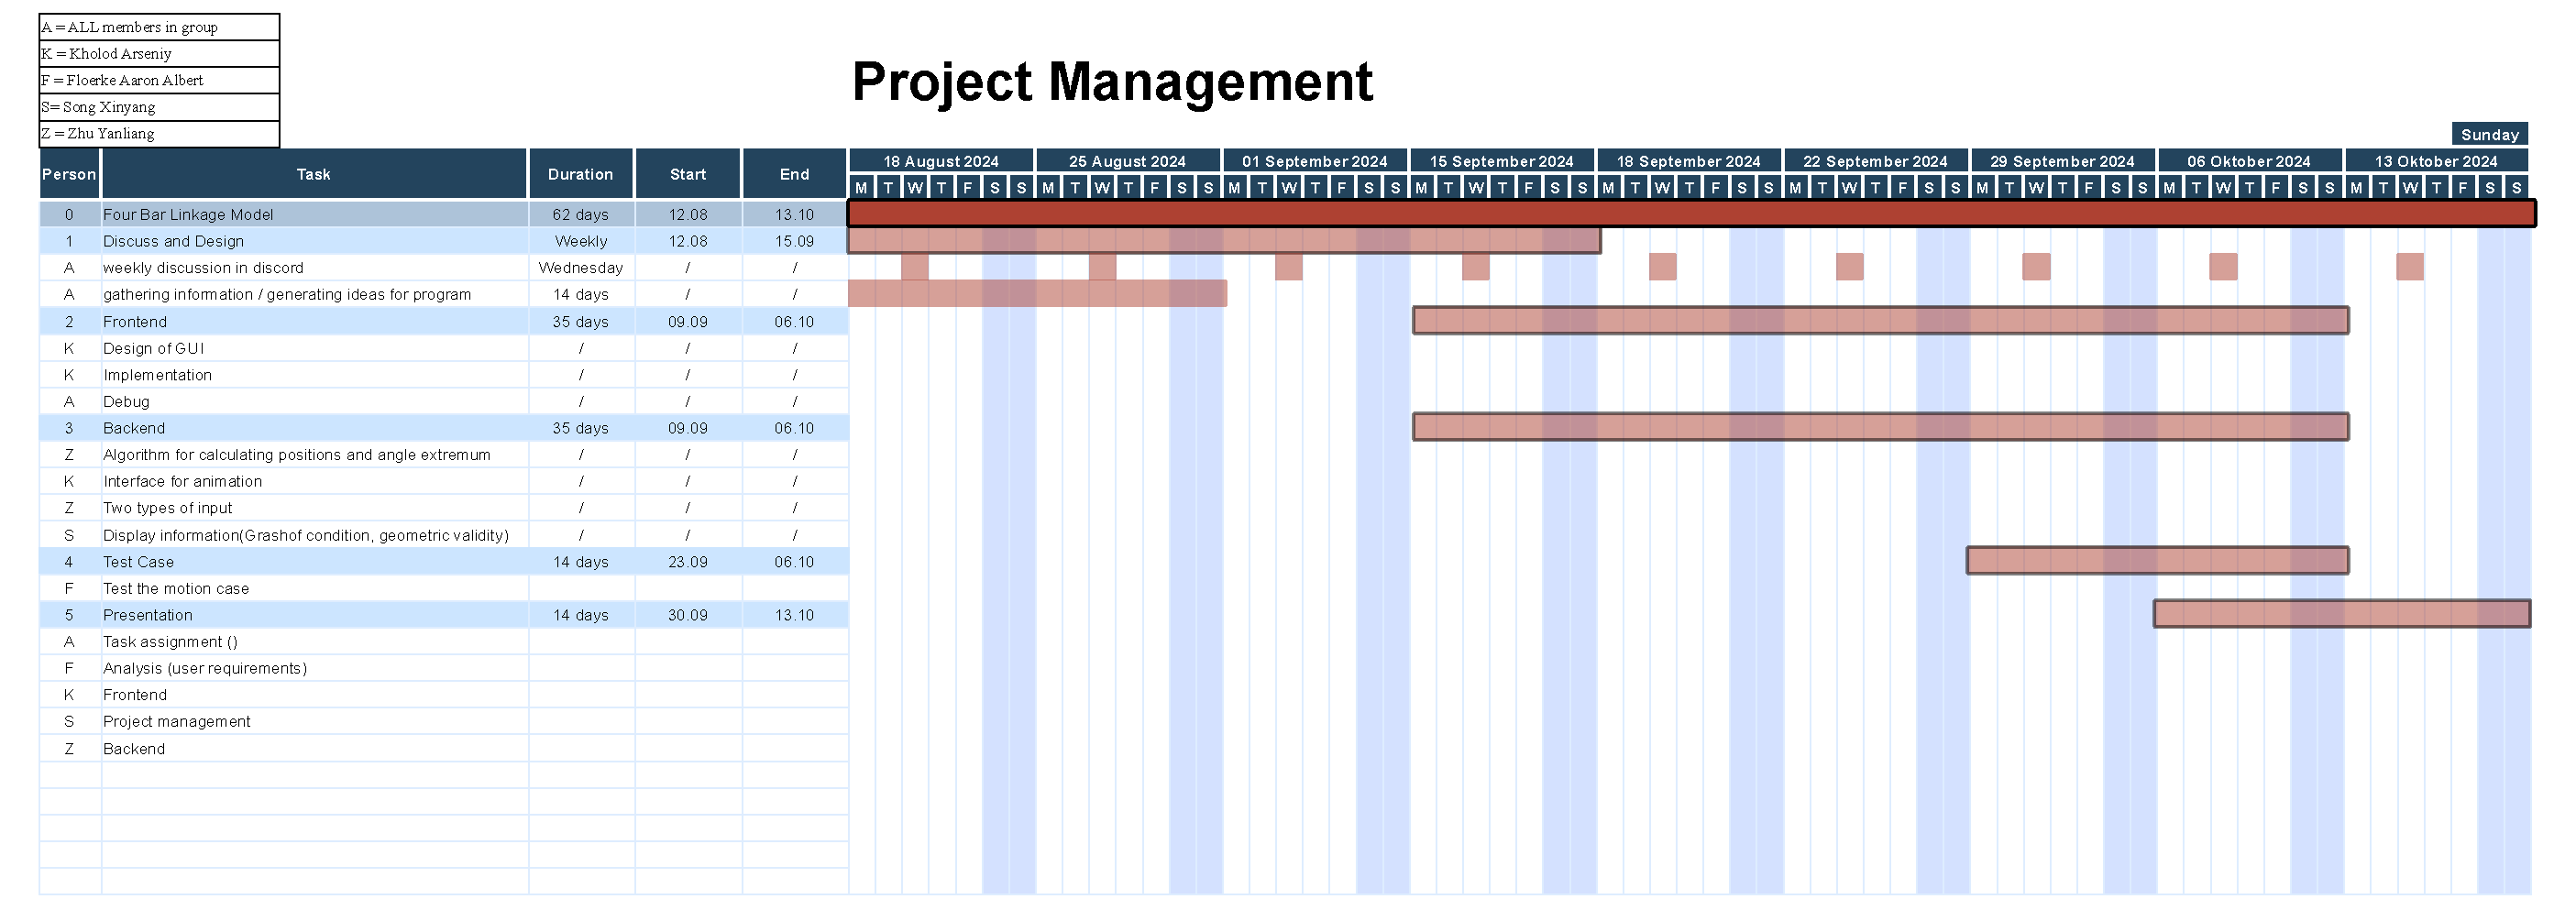
\includegraphics[width=\textwidth]{./figures/project_management_gantt_chart.pdf}
	\caption{Gantt Chart for Project Management}
	\label{fig:project_management_gantt_chart}
\end{figure}

The front-end and back-end development of the four-bar linkage was carried out using the agile methodology, Scrum, which employs an incremental and iterative approach to ensure project completion. The team meetings were held at least once every two weeks for planning the next and reviewing the previous tasks. We implemented features step by step and conducted testing accordingly as planned.

The following list is the specific task allocation for each group member:

\begin{itemize}
    \item Arseniy Kholod: The leader of the team, responsible for front-end development and task assignment.
    \item Yanliang Zhu: Responsible for back-end development.
    \item Aaron Albert Floerke: Responsible for testing.
    \item Xinyang Song: Responsible for code documentation.
\end{itemize}

Below is an overview of team collaboration and progress:
\begin{itemize}
    \item The first goal was to implement a basic static visualization of the four-bar linkage. Arseniy used tkinter to create the GUI. Zhu added functions such as joints' position calculation and validation of the input parameters to the back-end.
    \item In mid-August, Aaron introduced Python's unit testing to test 27 different motion types.
    \item By mid-September, we completed the function for animation. However, Zhu encountered issues with switching between $C_1$ and $C_2$ in the back-end in specific cases.
    \item Arseniy raised an issue on GitHub and solved the switching problem. Afterward, he added several new features to the front-end, such as tracing of joints.
    \item In early October, our team solved the optimization problem. After the presentation in October, we began preparing the final report.
\end{itemize}

\section{Conclusions}

Over the last several months, we successfully completed the "Pusher Mechanism" project. This included analyzing user requirements, deriving system requirements, establishing a theoretical foundation for the four-bar linkage, designing and implementing the software and test cases, validating the system's accuracy and solving the defined optimization problem.

The most challenging part of this project was the project management. Organizing the team, efficiently distributing tasks, and integrating all software components together were the critical parts. But despite the challenges, we are proud to successfully manage them.

While we are satisfied with the results, there is room for improvement. Although we developed software to validate the solution of the optimization problem, we did not implement an automated algorithm to efficiently determine such solutions. Developing such an algorithm would be a logical next step for this project.

\bibliographystyle{plain}
\bibliography{literature}

\appendix

\section{Animation UML State Diagram} \label{ap:animation}

\begin{figure}[h]
	\centering
	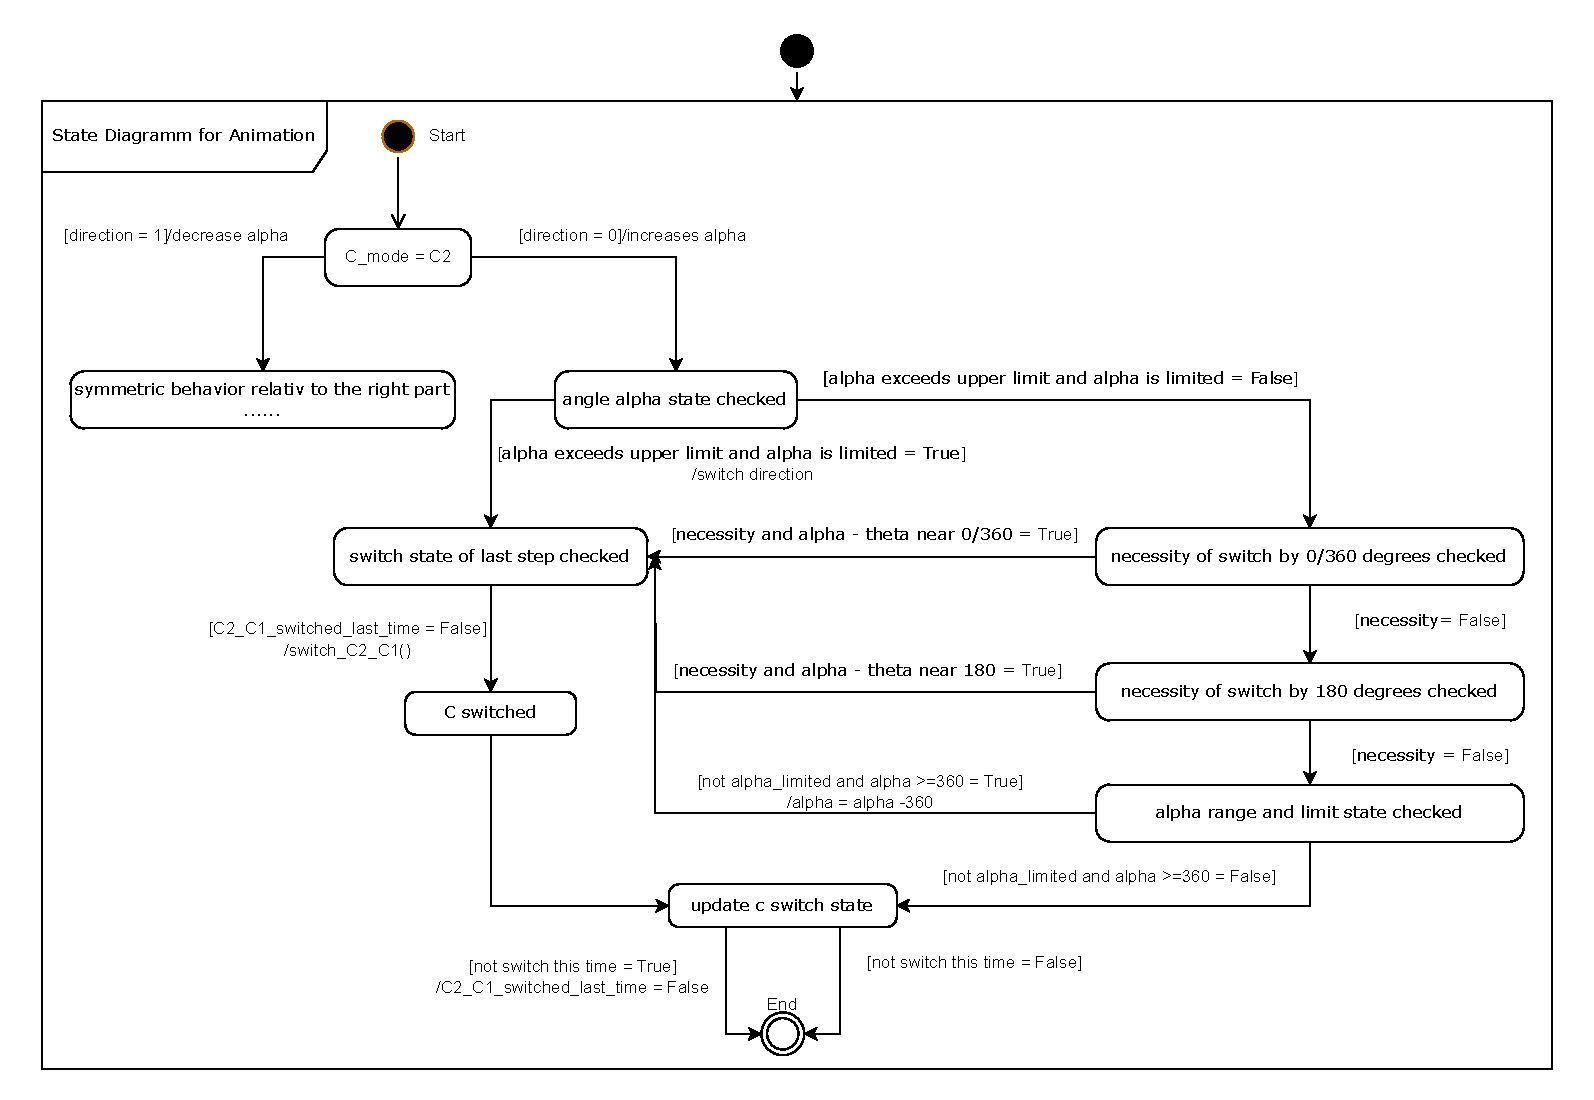
\includegraphics[width=\textwidth]{./figures/animation_state_diagramm_1.pdf}
	\caption{State Diagramm for Animation}
	\label{fig:state_diagramm_of_animation_alpha}
\end{figure}

\section{User Documentation} \label{ch:user_docs}

\subsection{Installation}

Install Python\footnote{\url{https://www.python.org/downloads/}} and Python's libraries: tkinter\footnote{\url{https://docs.python.org/3/library/tkinter.html}}, numpy\footnote{\url{https://numpy.org/}}, math\footnote{\url{https://docs.python.org/3/library/math.html}}, and unittest\footnote{\url{https://docs.python.org/3/library/unittest.html}}. Note that tkinter, math and unittest are pre-installed with Python, while numpy needs to be installed separately.

\subsection{Running}

Download the gui.py\footnote{\url{https://github.com/einsflash/Project_Pusher_Mechanism/blob/main/src/gui.py}} and four\_bar\_linkage.py\footnote{\url{https://github.com/einsflash/Project_Pusher_Mechanism/blob/main/src/four_bar_linkage.py}} files in the same directory. Start the GUI by calling the following.

\begin{lstlisting}[language=bash]
$ python ./gui.py
\end{lstlisting}

\subsection{Testing}

Download the following files in the same directory: 27Test.py\footnote{\url{https://github.com/einsflash/Project_Pusher_Mechanism/blob/main/src/27Test.py}} and motionTestCases.py\footnote{\url{https://github.com/einsflash/Project_Pusher_Mechanism/blob/main/src/motionTestCases.py}}. Test the software by calling:

\begin{lstlisting}[language=bash]
$ python ./motionTestCases.py
$ python ./27Test.py
\end{lstlisting}


\section{Screenshots}

\begin{figure}[h]
	\centering
	\begin{subfigure}{0.7\textwidth}
		\centering
		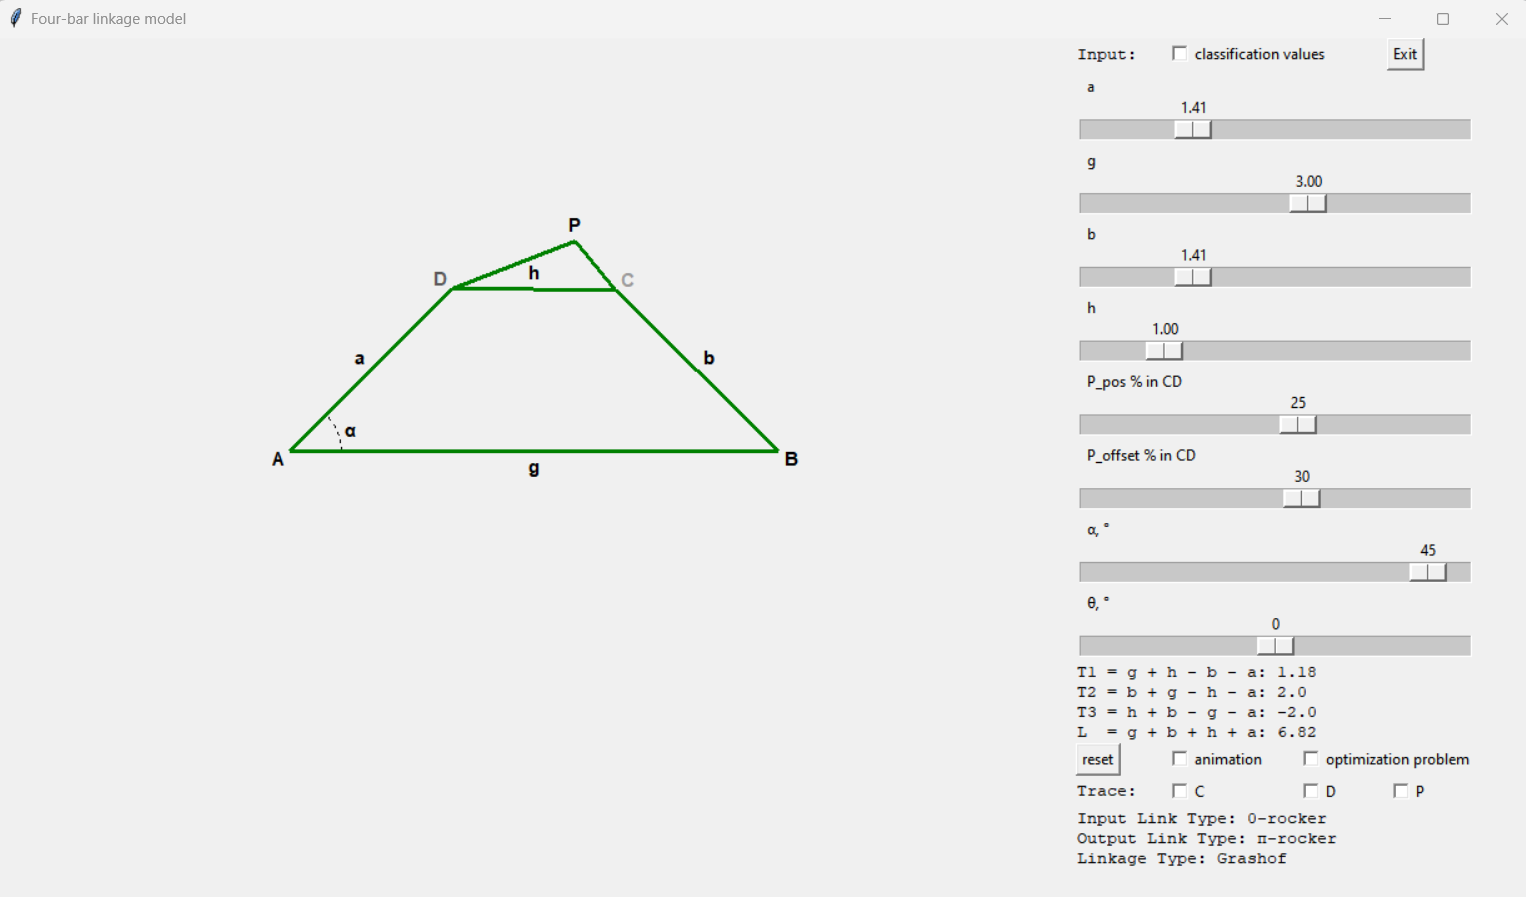
\includegraphics[width=\linewidth]{./figures/GUI_screenshots/GUI_default.png}
		\caption{GUI, default.}
		\label{fig:GUI_default}
	\end{subfigure}
	\vfill
	\begin{subfigure}{0.7\textwidth}
		\centering
		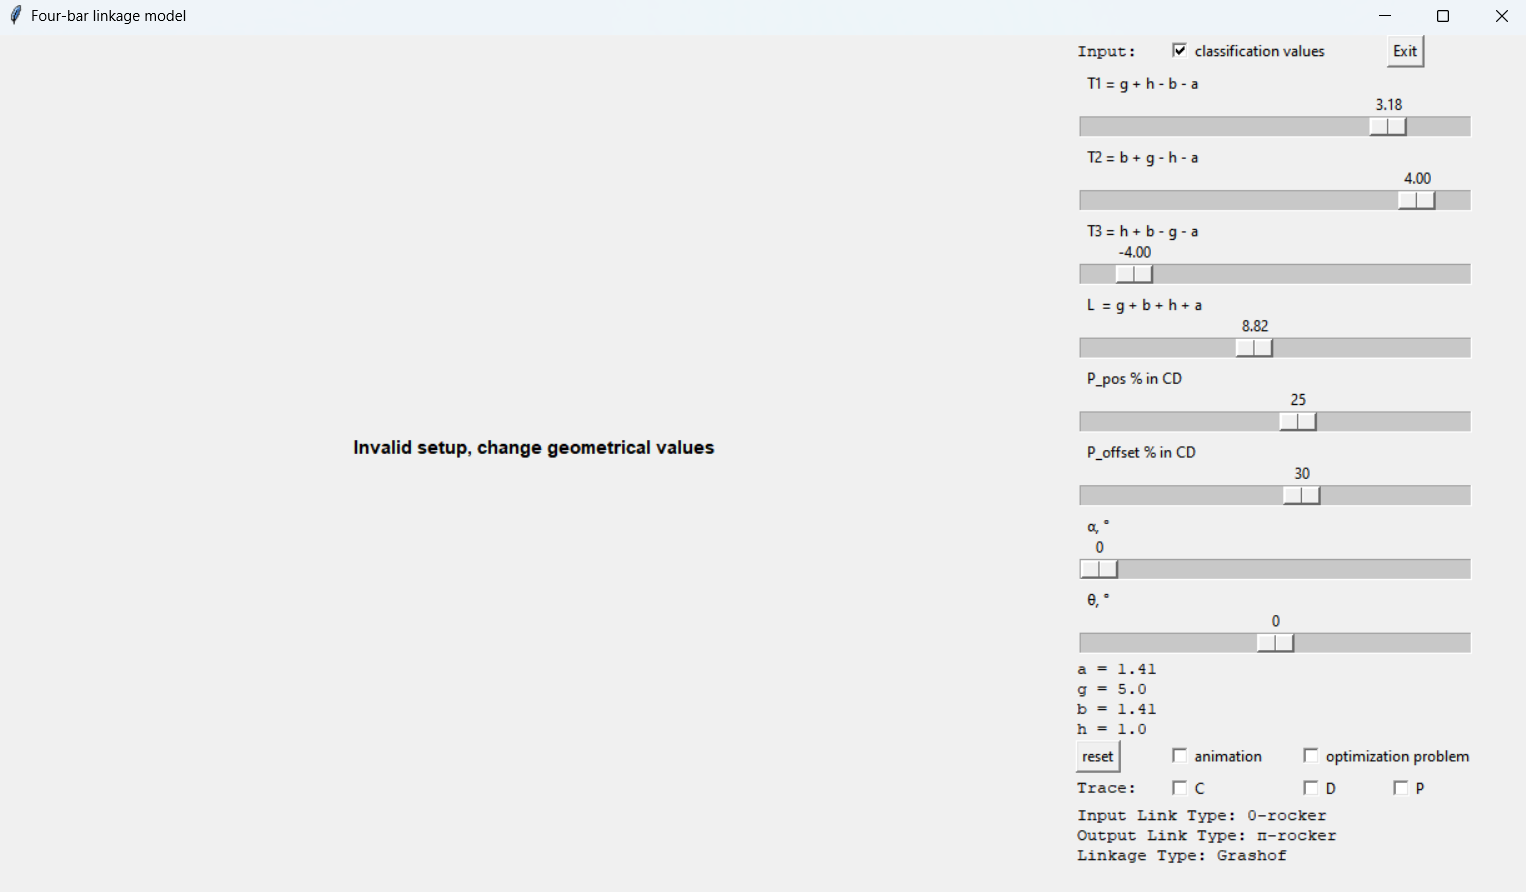
\includegraphics[width=\linewidth]{./figures/GUI_screenshots/GUI_invalid_setup.png}
		\caption{GUI, invalid setup and classification values as the input.}
		\label{fig:GUI_invalid}
	\end{subfigure}
	\vfill
	\begin{subfigure}{0.7\textwidth}
		\centering
		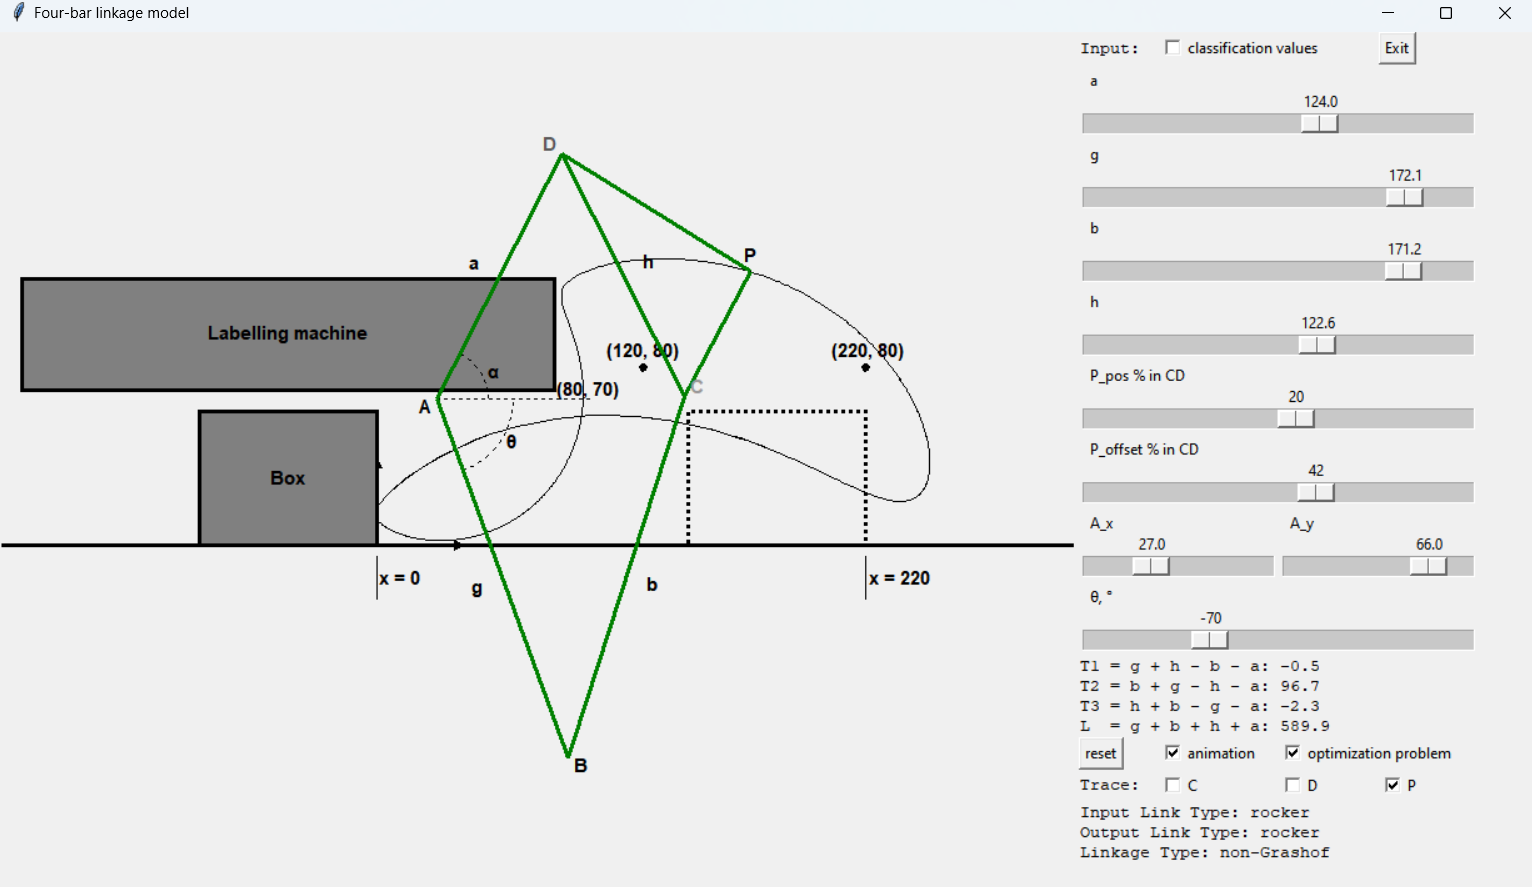
\includegraphics[width=\linewidth]{./figures/GUI_screenshots/GUI_optimization_problem.png}
		\caption{GUI, animation, tracing and optimization problem.}
		\label{fig:GUI_optimization_problem}
	\end{subfigure}
	\caption{GUI screenshots}
\end{figure}

\begin{figure}[h]
	\centering
	\begin{subfigure}{0.19\textwidth}
		\centering
		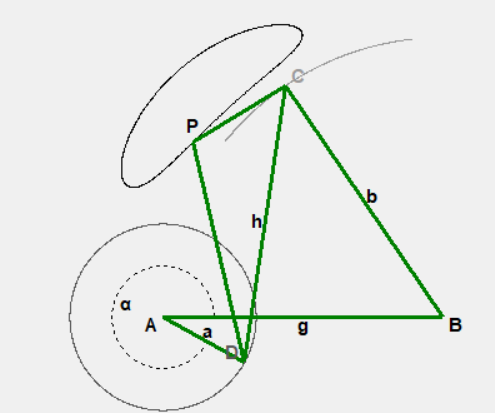
\includegraphics[width=\linewidth, height=0.95\linewidth, keepaspectratio]{./Figures/27_motion_cases/111.png}
		\caption{\scalebox{0.8}{$T_{1,2,3} = 1, 1, 1$}}
	\end{subfigure}
	\hfill
	\begin{subfigure}{0.19\textwidth}
		\centering
		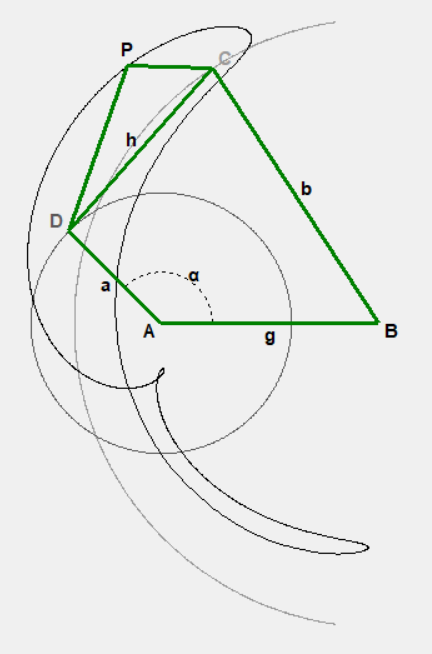
\includegraphics[width=\linewidth, height=0.95\linewidth, keepaspectratio]{./Figures/27_motion_cases/011.png}
		\caption{\scalebox{0.8}{$T_{1,2,3} = 0, 1, 1$}}
	\end{subfigure}
	\hfill
	\begin{subfigure}{0.19\textwidth}
		\centering
		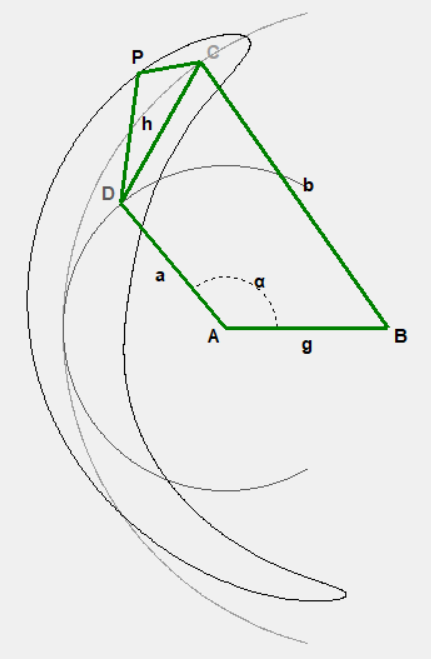
\includegraphics[width=\linewidth, height=0.95\linewidth, keepaspectratio]{./Figures/27_motion_cases/-111.png}
		\caption{\scalebox{0.8}{$T_{1,2,3} = -1, 1, 1$}}
	\end{subfigure}
	\hfill
	\begin{subfigure}{0.19\textwidth}
		\centering
		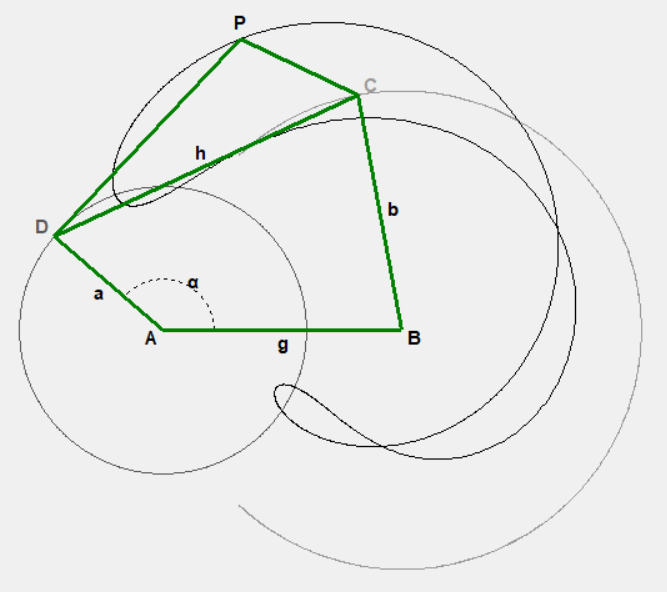
\includegraphics[width=\linewidth, height=0.95\linewidth, keepaspectratio]{./Figures/27_motion_cases/101.png}
		\caption{\scalebox{0.8}{$T_{1,2,3} = 1, 0, 1$}}
	\end{subfigure}
	\hfill
	\begin{subfigure}{0.19\textwidth}
		\centering
		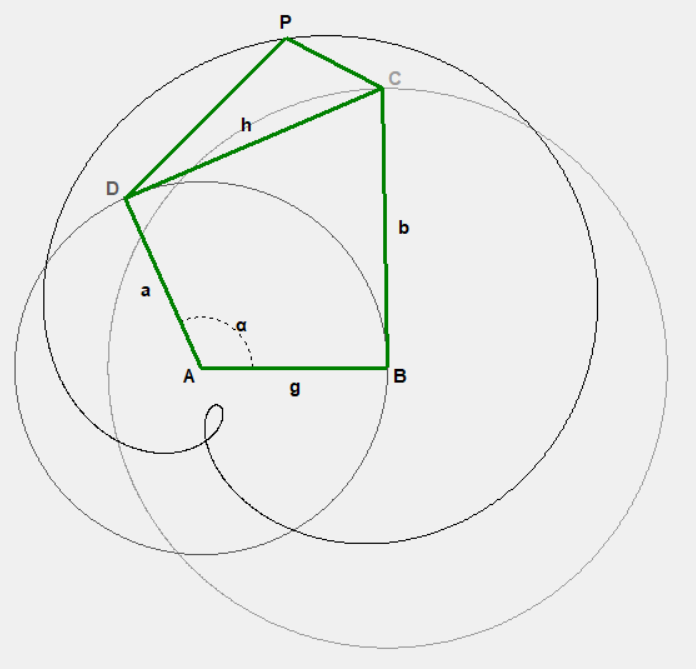
\includegraphics[width=\linewidth, height=0.95\linewidth, keepaspectratio]{./Figures/27_motion_cases/001.png}
		\caption{\scalebox{0.8}{$T_{1,2,3} = 0, 0, 1$}}
	\end{subfigure}
	\vfill
	\begin{subfigure}{0.19\textwidth}
		\centering
		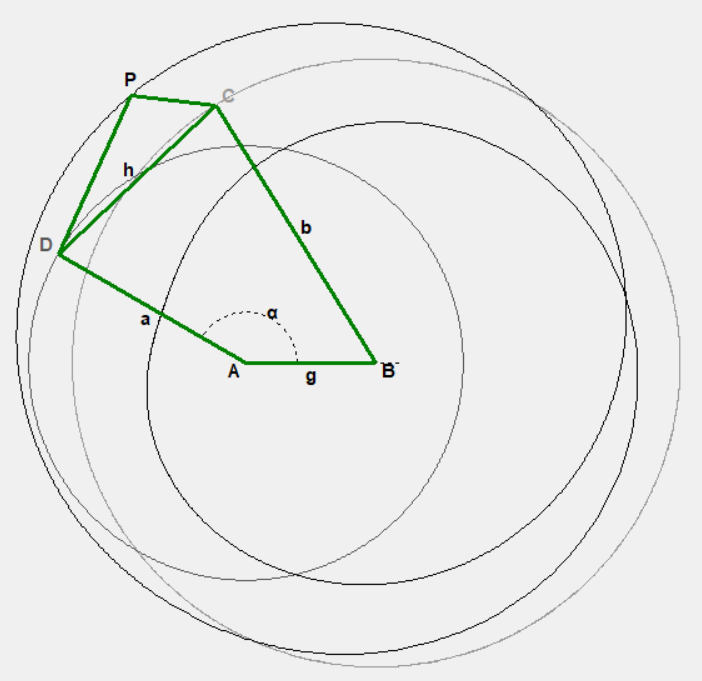
\includegraphics[width=\linewidth, height=0.95\linewidth, keepaspectratio]{./Figures/27_motion_cases/-101.png}
		\caption{\scalebox{0.8}{$T_{1,2,3} = =1, 0, 1$}}
	\end{subfigure}
	\hfill
	\begin{subfigure}{0.19\textwidth}
		\centering
		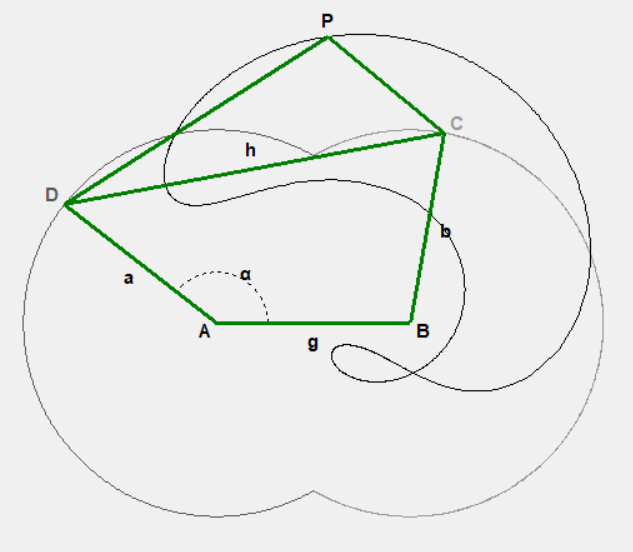
\includegraphics[width=\linewidth, height=0.95\linewidth, keepaspectratio]{./Figures/27_motion_cases/1-11.png}
		\caption{\scalebox{0.8}{$T_{1,2,3} = 1, -1, 1$}}
	\end{subfigure}
	\hfill
	\begin{subfigure}{0.19\textwidth}
		\centering
		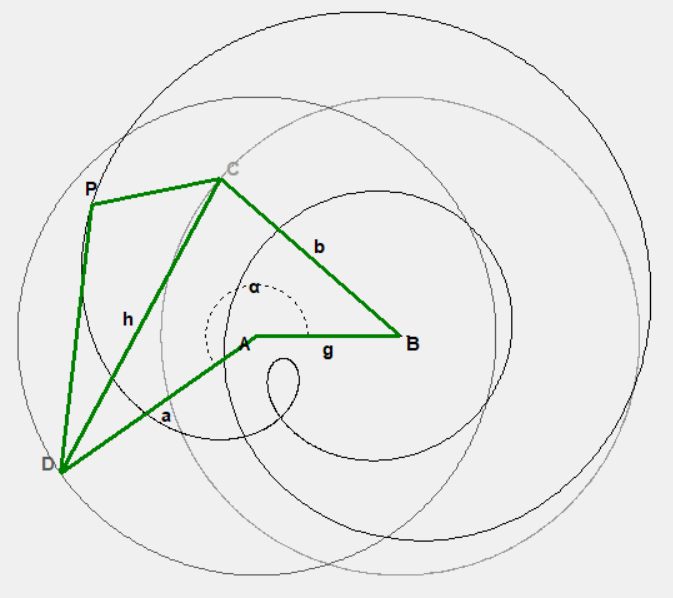
\includegraphics[width=\linewidth, height=0.95\linewidth, keepaspectratio]{./Figures/27_motion_cases/0-11.png}
		\caption{\scalebox{0.8}{$T_{1,2,3} = 0, -1, 1$}}
	\end{subfigure}
	\hfill
	\begin{subfigure}{0.19\textwidth}
		\centering
		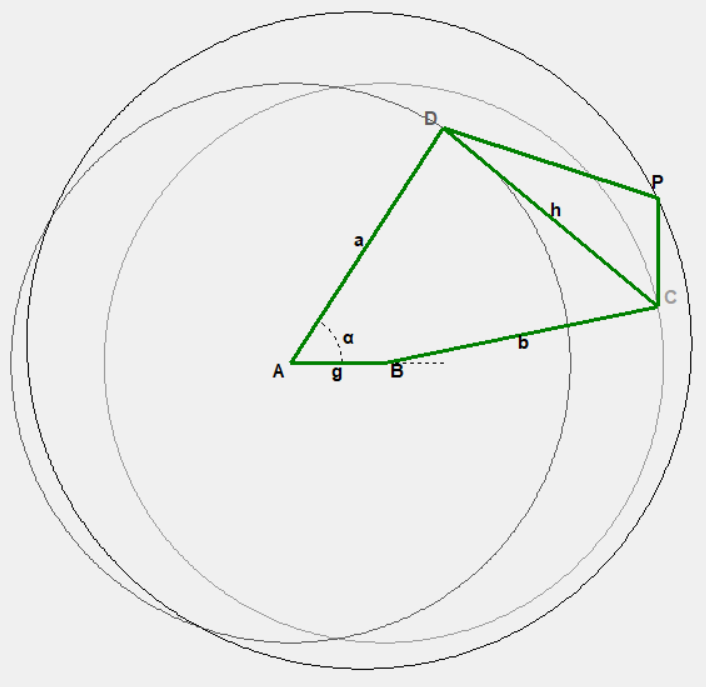
\includegraphics[width=\linewidth, height=0.95\linewidth, keepaspectratio]{./Figures/27_motion_cases/-1-11.png}
		\caption{\scalebox{0.8}{$T_{1,2,3} = -1, -1, 1$}}
	\end{subfigure}
	\hfill
	\begin{subfigure}{0.19\textwidth}
		\centering
		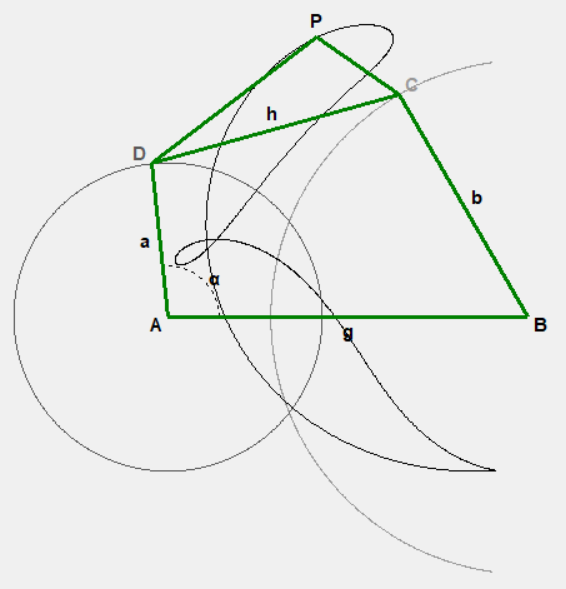
\includegraphics[width=\linewidth, height=0.95\linewidth, keepaspectratio]{./Figures/27_motion_cases/110.png}
		\caption{\scalebox{0.8}{$T_{1,2,3} = 1, 1, 0$}}
	\end{subfigure}
	\vfill
	\begin{subfigure}{0.19\textwidth}
		\centering
		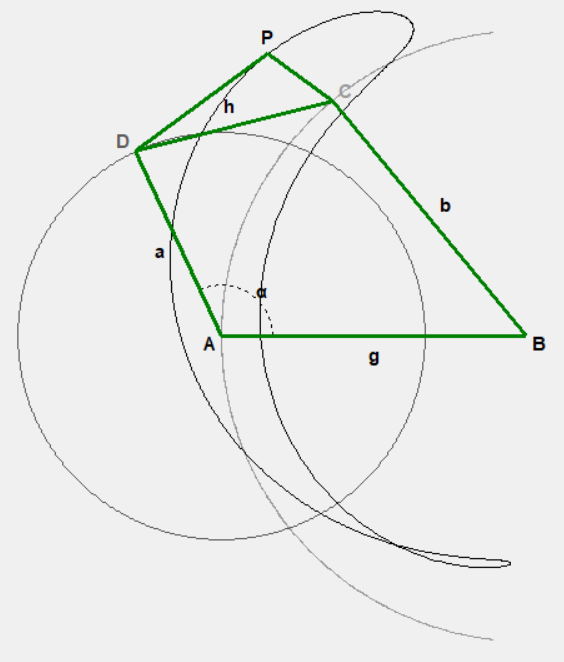
\includegraphics[width=\linewidth, height=0.95\linewidth, keepaspectratio]{./Figures/27_motion_cases/010.png}
		\caption{\scalebox{0.8}{$T_{1,2,3} = 0, 1, 0$}}
	\end{subfigure}
	\hfill
	\begin{subfigure}{0.19\textwidth}
		\centering
		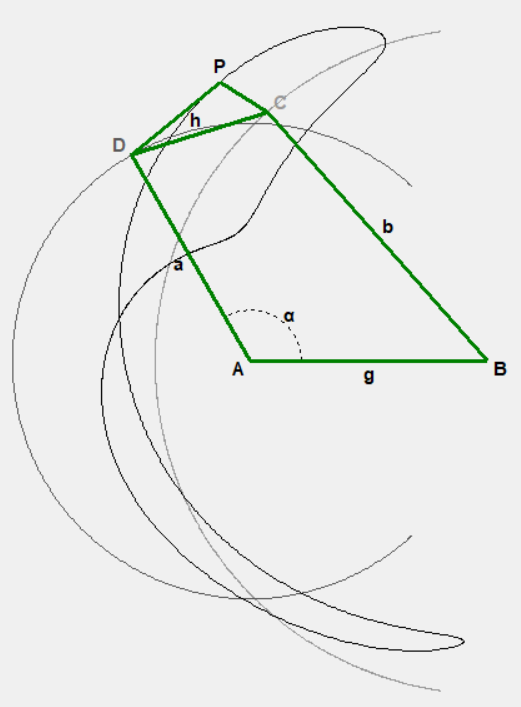
\includegraphics[width=\linewidth, height=0.95\linewidth, keepaspectratio]{./Figures/27_motion_cases/-110.png}
		\caption{\scalebox{0.8}{$T_{1,2,3} = -1, 1, 0$}}
	\end{subfigure}
	\hfill
	\begin{subfigure}{0.19\textwidth}
		\centering
		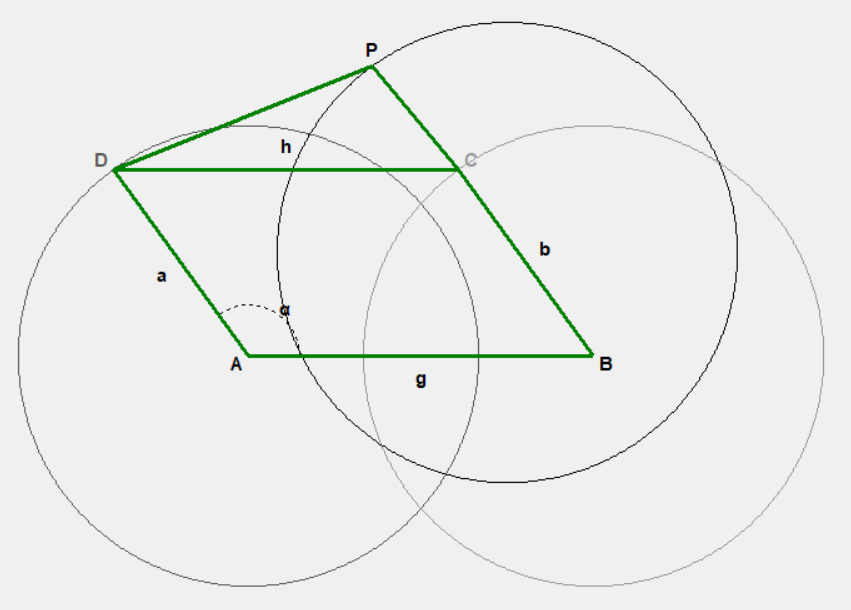
\includegraphics[width=\linewidth, height=0.95\linewidth, keepaspectratio]{./Figures/27_motion_cases/100.png}
		\caption{\scalebox{0.8}{$T_{1,2,3} = 1, 0, 0$}}
	\end{subfigure}
	\hfill
	\begin{subfigure}{0.19\textwidth}
		\centering
		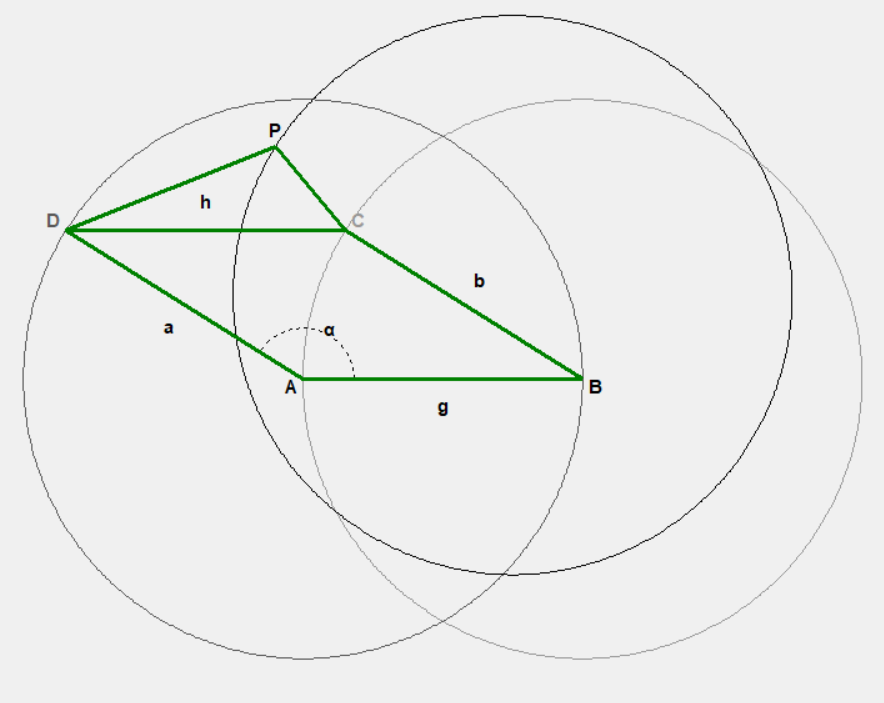
\includegraphics[width=\linewidth, height=0.95\linewidth, keepaspectratio]{./Figures/27_motion_cases/000.png}
		\caption{\scalebox{0.8}{$T_{1,2,3} = 0, 0, 0$}}
	\end{subfigure}
	\hfill
	\begin{subfigure}{0.19\textwidth}
		\centering
		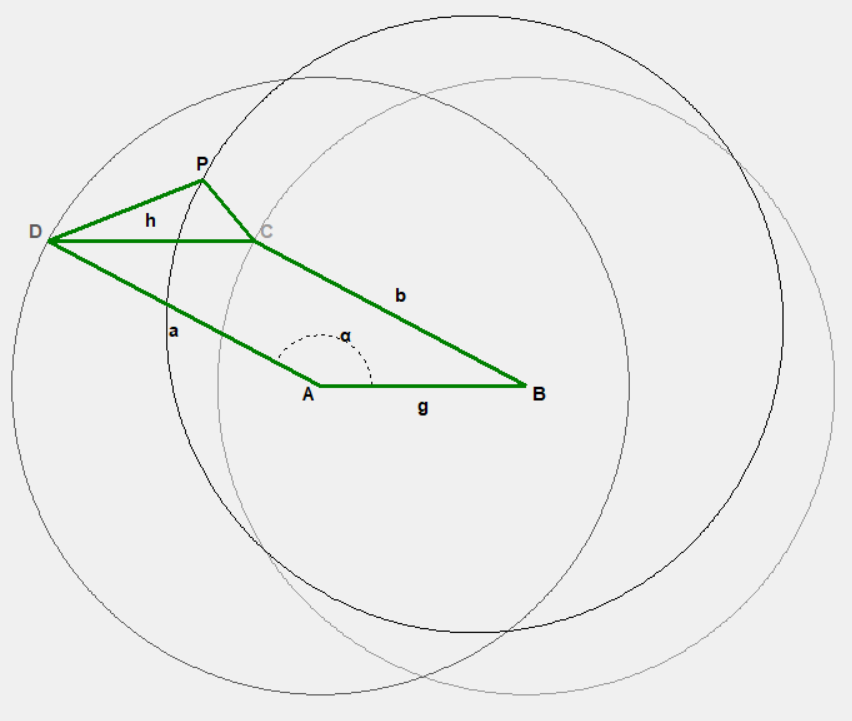
\includegraphics[width=\linewidth, height=0.95\linewidth, keepaspectratio]{./Figures/27_motion_cases/-100.png}
		\caption{\scalebox{0.8}{$T_{1,2,3} = -1, 0, 0$}}
	\end{subfigure}
	\vfill
	\begin{subfigure}{0.19\textwidth}
		\centering
		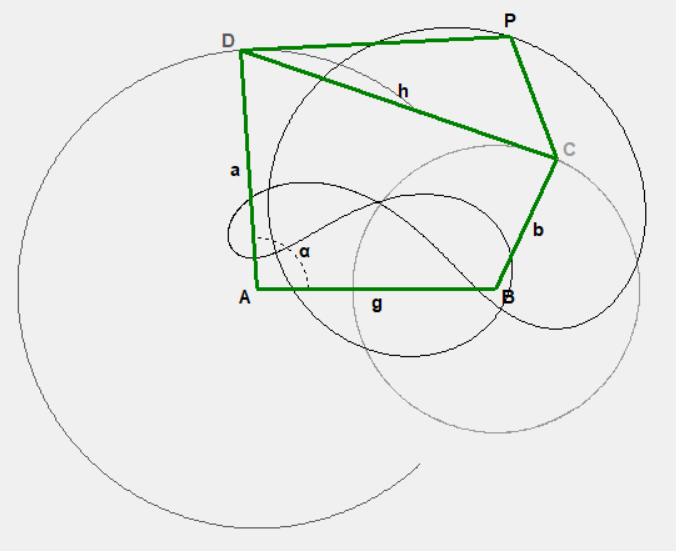
\includegraphics[width=\linewidth, height=0.95\linewidth, keepaspectratio]{./Figures/27_motion_cases/1-10.png}
		\caption{\scalebox{0.8}{$T_{1,2,3} = 1, -1, 0$}}
	\end{subfigure}
	\hfill
	\begin{subfigure}{0.19\textwidth}
		\centering
		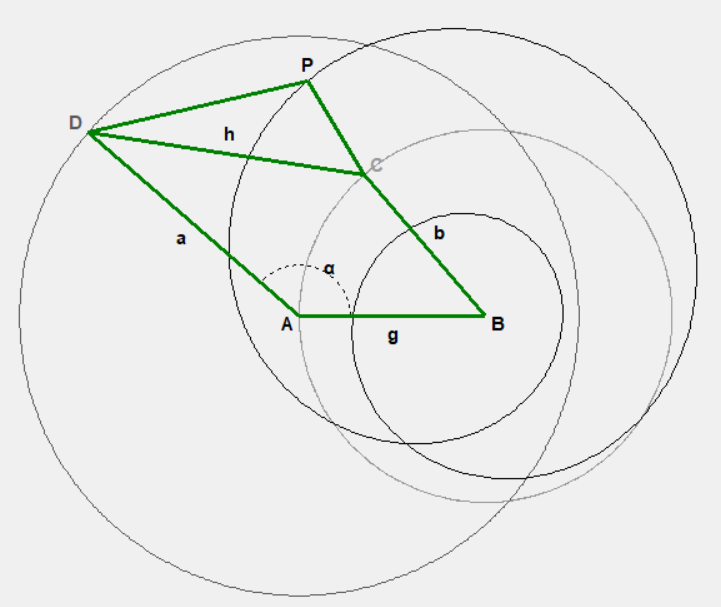
\includegraphics[width=\linewidth, height=0.95\linewidth, keepaspectratio]{./Figures/27_motion_cases/0-10.png}
		\caption{\scalebox{0.8}{$T_{1,2,3} = 0, -1, 0$}}
	\end{subfigure}
	\hfill
	\begin{subfigure}{0.19\textwidth}
		\centering
		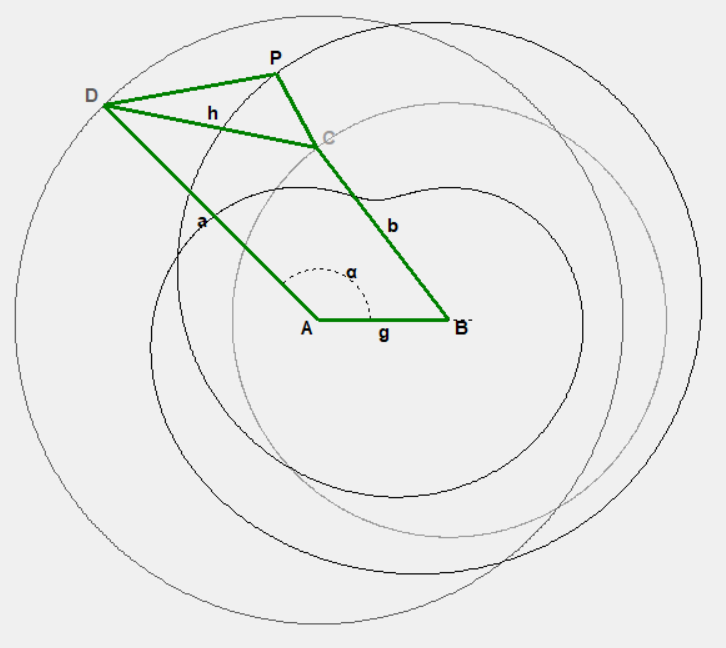
\includegraphics[width=\linewidth, height=0.95\linewidth, keepaspectratio]{./Figures/27_motion_cases/-1-10.png}
		\caption{\scalebox{0.8}{$T_{1,2,3} = -1, -1, 0$}}
	\end{subfigure}
	\hfill
	\begin{subfigure}{0.19\textwidth}
		\centering
		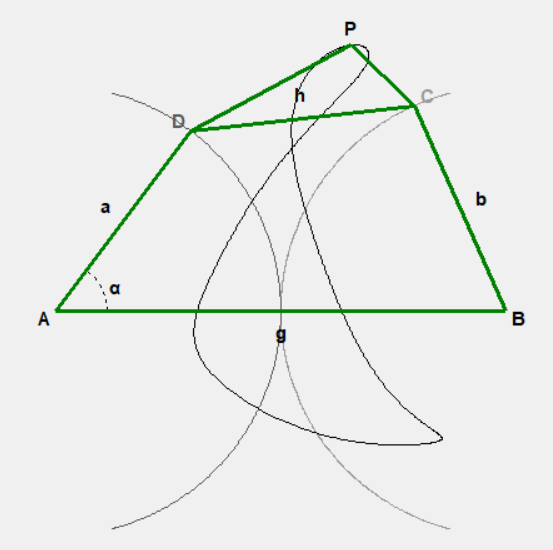
\includegraphics[width=\linewidth, height=0.95\linewidth, keepaspectratio]{./Figures/27_motion_cases/11-1.png}
		\caption{\scalebox{0.8}{$T_{1,2,3} = 1, 1, -1$}}
	\end{subfigure}
	\hfill
	\begin{subfigure}{0.19\textwidth}
		\centering
		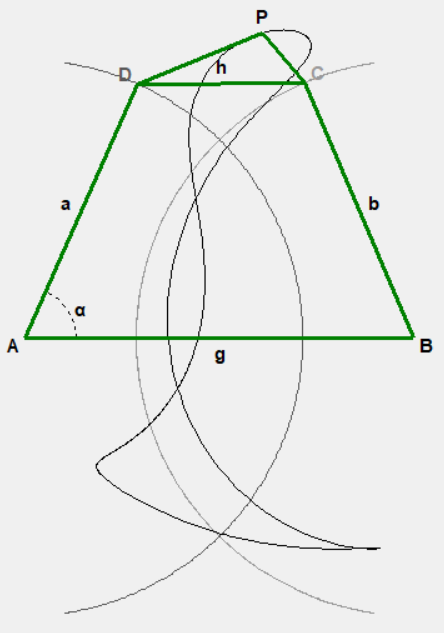
\includegraphics[width=\linewidth, height=0.95\linewidth, keepaspectratio]{./Figures/27_motion_cases/01-1.png}
		\caption{\scalebox{0.8}{$T_{1,2,3} = 0, 1, -1$}}
	\end{subfigure}
	\vfill
	\begin{subfigure}{0.19\textwidth}
		\centering
		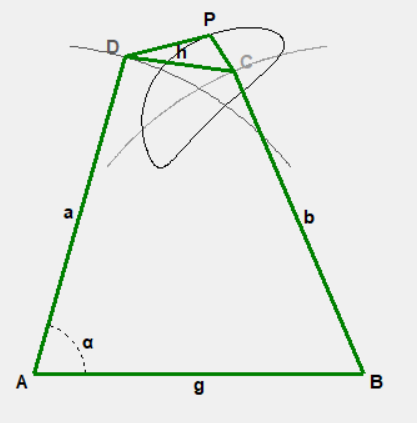
\includegraphics[width=\linewidth, height=0.95\linewidth, keepaspectratio]{./Figures/27_motion_cases/-11-1.png}
		\caption{\scalebox{0.8}{$T_{1,2,3} = -1, 1, -1$}}
	\end{subfigure}
	\hfill
	\begin{subfigure}{0.19\textwidth}
		\centering
		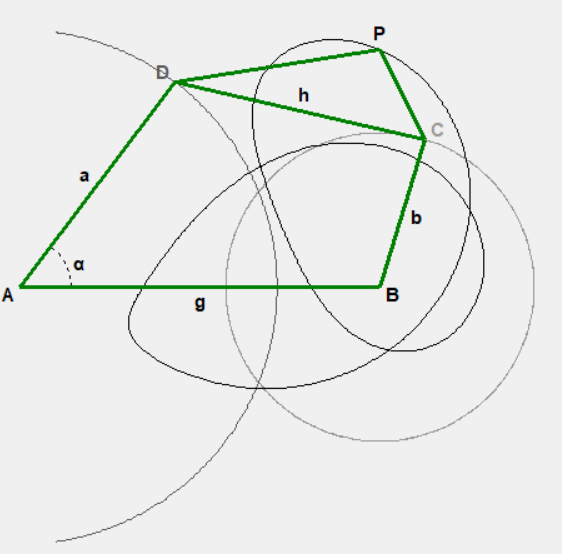
\includegraphics[width=\linewidth, height=0.95\linewidth, keepaspectratio]{./Figures/27_motion_cases/10-1.png}
		\caption{\scalebox{0.8}{$T_{1,2,3} = 1, 0, -1$}}
	\end{subfigure}
	\hfill
	\begin{subfigure}{0.19\textwidth}
		\centering
		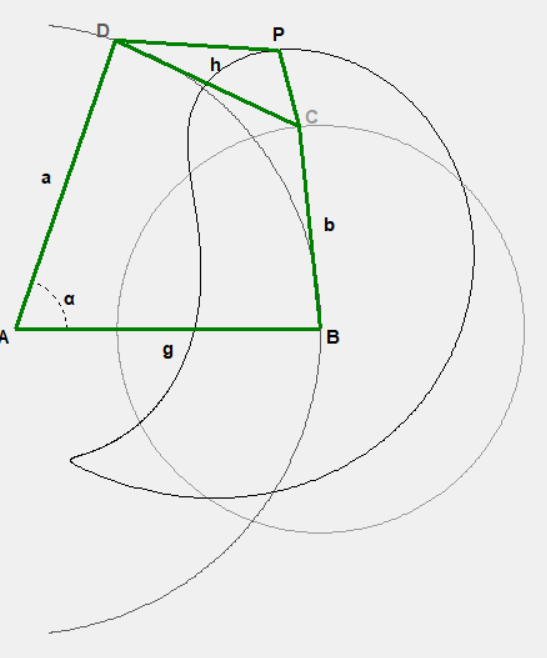
\includegraphics[width=\linewidth, height=0.95\linewidth, keepaspectratio]{./Figures/27_motion_cases/00-1.png}
		\caption{\scalebox{0.8}{$T_{1,2,3} = 0, 0, -1$}}
	\end{subfigure}
	\hfill
	\begin{subfigure}{0.19\textwidth}
		\centering
		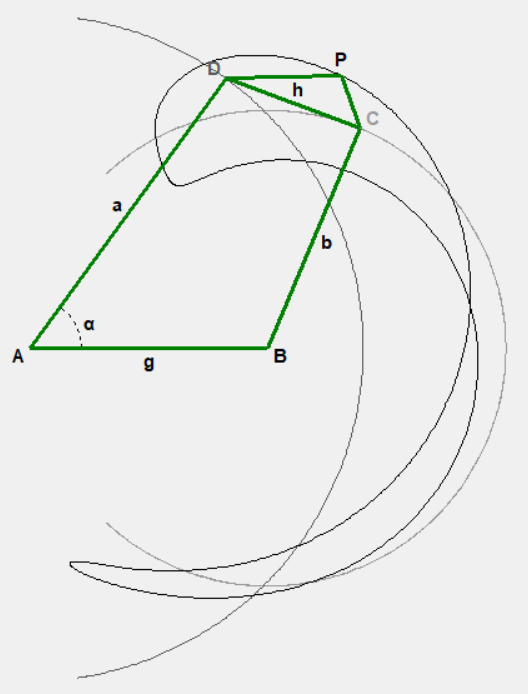
\includegraphics[width=\linewidth, height=0.95\linewidth, keepaspectratio]{./Figures/27_motion_cases/-10-1.png}
		\caption{\scalebox{0.8}{$T_{1,2,3} = -1, 0, -1$}}
	\end{subfigure}
	\hfill
	\begin{subfigure}{0.19\textwidth}
		\centering
		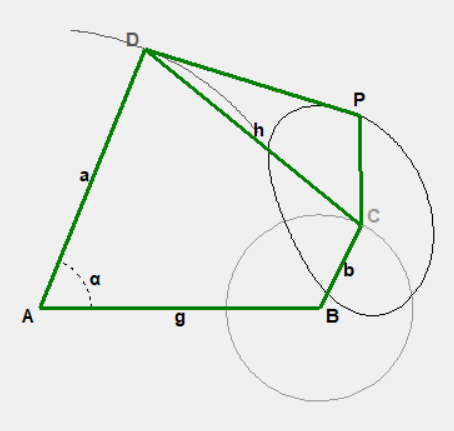
\includegraphics[width=\linewidth, height=0.95\linewidth, keepaspectratio]{./Figures/27_motion_cases/1-1-1.png}
		\caption{\scalebox{0.8}{$T_{1,2,3} = 1, -1, -1$}}
	\end{subfigure}
	\vfill
	\begin{subfigure}{0.19\textwidth}
		\centering
		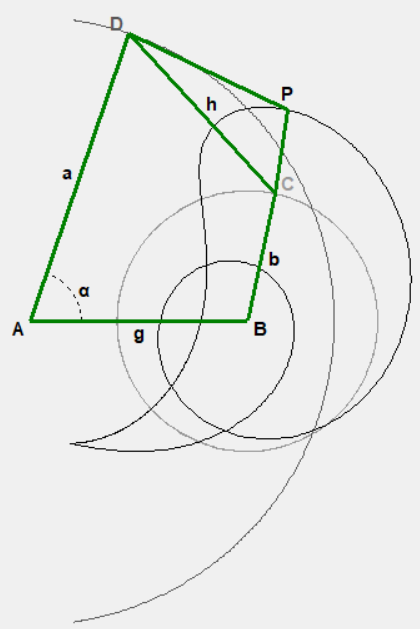
\includegraphics[width=\linewidth, height=0.95\linewidth, keepaspectratio]{./Figures/27_motion_cases/0-1-1.png}
		\caption{\scalebox{0.8}{$T_{1,2,3} = 0, -1, -1$}}
	\end{subfigure}
	\hfill
	\begin{subfigure}{0.19\textwidth}
		\centering
		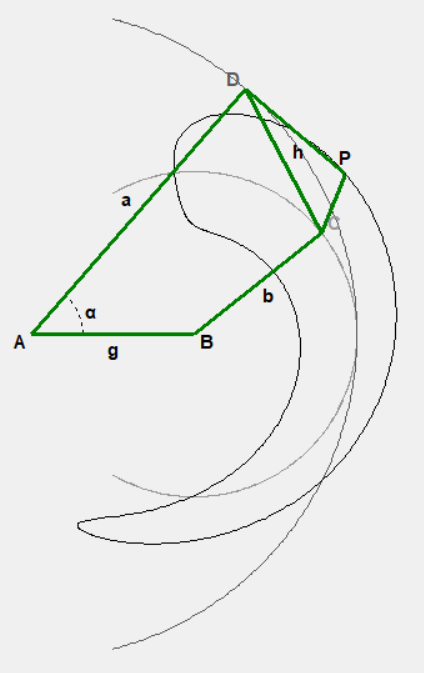
\includegraphics[width=\linewidth, height=0.95\linewidth, keepaspectratio]{./Figures/27_motion_cases/-1-1-1.png}
		\caption{\scalebox{0.8}{$T_{1,2,3} = -1, -1, -1$}}
	\end{subfigure}
	\caption{27 motion types.}
	\label{fig:27_motion_types}
\end{figure}


\end{document}

